\documentclass[utf8x,hyperref={pagebackref=true,citecolor=green,bookmarks=true,pdfpagelabels=false}]{beamer} %remove draft when done with tex prep

\usepackage{etex}
\usepackage{beamerthemesplit}
\usetheme{Berkeley} %Hannover, Belin, Warsaw, PaloAlto, Frankfurt, Berkeley  etc
\usepackage{pgfpages}
\mode<handout>{\setbeamercolor{background canvas sidebar}{bg=yellow!95}}

\usepackage{bm}
\usepackage{subfloat}
\usepackage{amssymb, amsmath}
\usepackage[round]{natbib}
\usepackage{algorithm}
\usepackage{algpseudocode}
\bibliographystyle{unsrtnat}
\usepackage[export]{adjustbox}
\usepackage{array,booktabs,tabularx}
\usepackage{tikz}
\usetikzlibrary{shapes,arrows, circuits, patterns, snakes, decorations.pathreplacing}
\usepackage{schemabloc, verbatim}
\usepackage{epstopdf}
\usepackage{graphicx}

%\graphicspath{../}  % path to base directory of all papers
\DeclareGraphicsExtensions{.eps}

\usepackage{media9} % for video embeddings
\usepackage{multimedia} % for video embeddings
\usepackage{tcolorbox}

%\usepackage[pagebackref=true,breaklinks=true,colorlinks=true, citecolor=green,linkcolor=cyan,urlcolor=blue,bookmarks=true]{hyperref}
%
%\usepackage[%pagebackref=true,breaklinks=true,colorlinks=true,
% citecolor=green,linkcolor=cyan,urlcolor=blue,bookmarks=true]{hyperref}
%
\newcommand{\tcb}[2]
{
 \begin{tcolorbox}[title=\text{#2}]
 #1
 \end{tcolorbox}
}

%\renewcommand\thefootnote{}\footnote{#1}
\definecolor{light-blue}{rgb}{0.30,0.35,1}
\definecolor{light-green}{rgb}{0.20,0.49,.85}
\definecolor{purple}{rgb}{0.70,0.69,.2}

\newcommand{\lb}[1]{\textcolor{light-blue}{#1}}
\newcommand{\bl}[1]{\textcolor{blue}{#1}}

\newcommand{\maybe}[1]{\textcolor{gray}{\textbf{MAYBE: }{#1}}}
\newcommand{\inspect}[1]{\textcolor{cyan}{\textbf{CHECK THIS: }{#1}}}
\newcommand{\more}[1]{\textcolor{red}{\textbf{MORE: }{#1}}}

% FYA
\newcommand{\cmt}[1]{{\footnotesize\textcolor{red}{#1}}}%{#2}
%\newcommand{\note}[1]{\cmt{Note: #1}}
%\newcommand{\todo}[1]{\textcolor{cyan}{TO-DO: #1}}
\newcommand{\review}[1]{\noindent\textcolor{red}{$\rightarrow$ #1}}
\newcommand{\response}[1]{\noindent{#1}}
\newcommand{\stopped}[1]{\color{red}STOPPED HERE #1\hrulefill}

%Text commands
\newcounter{mnote}
\newcommand{\marginote}[1]{\addtocounter{mnote}{1}\marginpar{\themnote. \scriptsize #1}}
\setcounter{mnote}{0}
% \newcommand{\comment}[1]{}
\newcommand{\ie}{$i.e.$\ }
\newcommand{\eg}{e.g.\ }
\newcommand{\cf}{c.f.\ }
\newcommand{\yes}{\checkmark}
\newcommand{\no}{\ding{55}}

%Reference commands
\newcommand{\flabel}[1]{\label{fig:#1}}
\newcommand{\seclabel}[1]{\label{sec:#1}}
\newcommand{\tlabel}[1]{\label{tab:#1}}
\newcommand{\elabel}[1]{\label{eq:#1}}
\newcommand{\alabel}[1]{\label{alg:#1}}
\newcommand{\fref}[1]{\cref{fig:#1}}
\newcommand{\sref}[1]{\cref{sec:#1}}
\newcommand{\tref}[1]{\cref{tab:#1}}
\newcommand{\eref}[1]{\cref{eq:#1}}
\newcommand{\aref}[1]{\cref{alg:#1}}

\newcommand{\bull}[1]{$\bullet$ #1}
\newcommand{\argmax}{\text{argmax}}
\newcommand{\argmin}{\text{argmin}}
\newcommand{\mc}[1]{\mathcal{#1}}
\newcommand{\bb}[1]{\mathbb{#1}}


\def\tidx{t}
%\def\comment
%\def\value{V}
% from https://www.cs.jhu.edu/~jason/advice/write-the-paper-first.html
\newcommand{\Note}[1]{}
\renewcommand{\Note}[1]{\hl{[#1]}}  % comment out this definition to suppress all Notes
%\algnewcommand\algorithmicforeach{\textbf{for each}}
%\algdef{S}[FOR]{Foreach}[1]{\algorithmicforeach\ #1\ \algorithmicdo} %

%\newcolumntype{M}[1]{>{\centering\arraybackslash}m{#1}}
\def\coriolis{\textbf{\textit{C}}}
\def\massinertia{\textbf{\textit{M}}}
\def\torque{\bm{\tau}}
\def\frictionvec{\textbf{\textit{f}}}
\def\Smat{\textbf{\textit{S}}}
\def\Bmat{\textbf{\textit{B}}}
\def\wheelrad{\textbf{\textit{r}}}

\def\stateweight{\textbf{\textit{w}}_x}
\def\actionweight{\textbf{\textit{w}}_u}
\def\advactionweight{\textbf{\textit{w}}_v}

%Thesis defs
%\def\upchi{\textchi}
\def\kau{\mc{K}}
\def\particle{\bm{x}}
\def\deformationgrad{\textbf{F}}
\def\refconf{\bm{\upchi}_0}
\def\refconfbody{\mathscr{B}_0}
\def\conf{\bm{\upchi}}
\def\currconf{\bm{\upchi}}
\def\Eulerian{\mc{E}}
\def\cauchystress{\bm{\sigma}}
\def\stresscomp{\sigma}
\def\currconfbody{\mathscr{B}}
\def\materialresponse{\textbf{G}}
\def\orthoggroup{{\textit{SO}}(3)}
\def\liegroup{{\textit{SE}}(3)}
\def\liealgebra{\mathfrak{se}(3)}
\def\identity{\textbf{I}}
\newcommand{\trace}[1]{\textbf{tr}(#1)}
\def\leftcauchy{\textbf{B}}
\def\rightcauchy{\textbf{C}}
\def\fiber{\textbf{dx}}

\def\dof{\text{DOF }}
\def\dofs{\text{DOFs }}
\def\reline{\mathbb{R}}
\def\curve{\deformationgrad}
\def\twist{{\xi}}
\def\contactforce{\tilde{F}}
\def\contactforcecomp{f}
\def\gaussianmap{\textbf{}n}
\def\contacttorquecomp{\tau}
\def\wrt{with respect to }
\def\curveparam{\position}
\def\basis{\bm{e}}
\def\pose{{g}}
\def\selmap{{B}}
\def\manipmap{{G}}
\def\jacob{\bm{J}}
\def\normal{\bm{n}}
\def\position{\textbf{r}}
\def\deformationgradcur{\textbf{H}}
\def\eulerianvel{\textbf{v}(\position, t)}
\def\headparam{\zeta}
\def\strain{\mathrm{\Psi}}
\def\strainiso{\mathrm{\Psi_{\text{iso}}}}
\def\strainfiber{\mathrm{\Psi_{\text{mesh}}}}

% mechanism defs
\def\wallthickness{1cm}
\def\sorodiam{9 cm}
\def\sorodiamdim{5-6.25cm}

% inline macros
\newcommand{\putsoro}[2]{\includegraphics[width=.45\columnwidth,height=#2\columnwidth]{../../../PhDThesis/figures/#1}}
\newcommand{\sorowidth}{.35}


%\newtheorem{theorem}{Theorem}[]
%\newtheorem{example}{Example}
%\newtheorem{homework}{Homework}

\tikzstyle{block} = [draw, fill=white!20, rectangle,minimum height=3em, minimum width=4em]
\tikzstyle{sum} = [draw, fill=white!20, circle, node distance=1cm]
\tikzstyle{input} = [coordinate]
\tikzstyle{output} = [coordinate]
\tikzstyle{pinstyle} = [pin edge={to-,thin,black}]

\newcolumntype{Z}{>{\centering\arraybackslash}X} % centered tabularx columns
\newcommand{\pphantom}{\textcolor{ta3aluminium}} % phantom
%\setbeamerfont{title}{shape=\itshape,family=\rmfamily}
\setbeamercolor{title}{fg=blue!70!black,bg=gray!40!white}
%
\title{\small A Multi-DOF Soft Robot Mechanism for Patient Motion Correction and 
		Beam Orientation Selection	in Cancer Radiation Therapy.
}
\author{Lekan Ogunmolu}
\institute{
	%
	\vspace{0.5em}
	%
	Department of Electrical Engineering \\
	The University of Texas at Dallas, Richardson, TX 
}

\date{May 16, 2019} 

\makeatletter
\setbeamertemplate{sidebar \beamer@sidebarside}%{sidebar theme}
{
	\beamer@tempdim=\beamer@sidebarwidth%
	\advance\beamer@tempdim by -6pt%
	\insertverticalnavigation{\beamer@sidebarwidth}%
	\vfill
	\ifx\beamer@sidebarside\beamer@lefttext%
	\else%
	\usebeamercolor{normal text}%
	\llap{\usebeamertemplate***{navigation symbols}\hskip0.1cm}%
	\vskip2pt%
	\fi%
}%
\makeatother
%PHONON=true
\begin{document}

\frame{\titlepage
}

\chapter{Preamble}
\label{chap:intro}

Consider this your roadmap for the course.  Please read through the syllabus posted on moodle carefully and feel free to share any questions that you may have.  Please print a copy of the syllabus for reference. Some relevant parts of the syllabus are repeated here but the moodle reference should serve as your guide throughout the ten weeks of this course.

\section{Course Description}
This course focuses on the algorithmic and mathematical concepts  with respect to robot planning, manipulation and control. Topics covered include kinematics and dynamics, as well as path planning and deep reinforcement learning algorithms. Simulations and experiments on hardware testbeds (listed in the syllabus) will be performed to test the related algorithms.

\section{Course Outcomes}
After taking this course, each student will be able to

\begin{itemize}
\item Develop planning and manipulation schemes to drive robot operation

\item Integrate perception algorithms into manipulation and planning systems

\item Determine the kinematic description of a robot's motion or locomotion
\end{itemize}

\section{Prerequisites}

RBOT 210 or an advanced knowledge of ROS; undergraduate-level experience or equivalent with object oriented programming; strong programming knowledge in Python and C++ is required; and RBOT 205 if mathematical foundational skills of admissions criteria are needed.

\section{Recommended Texts}
\begin{itemize}
	\item  	Main Texts
	\begin{itemize}
		\item Murray, R. M., Li, Z., and Sastry, S. S. (1994). A Mathematical Introduction to Robotic Manipulation. Book (Vol. 29). Free PDF preprint downloadable from, \href{https://www.cds.caltech.edu/~murray/books/MLS/pdf/mls94-complete.pdf }{Murray's website}.
		%
		\item 	Spong, M. W., Hutchinson, S., and Vidyasagar, M. (2012). Robot Modeling and Control. Students can buy from this \href{https://www.amazon.com/Robot-Modeling-Control-Mark-Spong/dp/0471649902}{Amazon Link}.
	\end{itemize} 
	%
	\item Secondary Text
	%
	\begin{itemize}
		\item Modern Robotics: Mechanics, Planning, and Control. Free PDF preprint downloadable from \href{ http://hades.mech.northwestern.edu/images/7/7f/MR.pdf}{Author's Northwestern Website}.		
	\end{itemize} 
    %
    \item 
    Auxiliary Text: 
    %
    \begin{itemize}
    	\item Theory of Screws: A Study in the Dynamics of a Rigid Body by Robert Stawell Ball, Dublin: Hodges, Foster, and Co., Grafton-Street (Should be downloadable via Interlibrary Loan).
    \end{itemize}
\end{itemize}

\section{Recommended Journals}
	%
	\begin{itemize}
		\item 
		\href{ https://ieeexplore.ieee.org/xpl/RecentIssue.jsp?punumber=8860}{IEEE Transactions on Robotics}.
		%
		\item 
		\href{https://journals.sagepub.com/home/ijr}{The International Journal of Robotics Research}.
		%
		\item 
		\href{https://www.ieee-ras.org/conferences-workshops/fully-sponsored/icra}{The IEEE International Conference on Robotics and Automation}.
		%
		\item \href{https://www.ieee-ras.org/conferences-workshops/financially-co-sponsored/iros}{IEEE/Robotics Society of Japan International Conference on Intelligent Robots and Systems (IROS)}.
		%
		\item \href{https://www.journals.elsevier.com/robotics-and-autonomous-systems}{Robotics and Autonomous Systems, An Elsevier Journal}.
	\end{itemize}

\section{Required Software}
	
	\begin{itemize}
	%
	\item A working knowledge of python and the anaconda environment.
	%
	\item \href{https://www.ros.org/}{The Robot Operating System}.
	%
	\item ROS from Conda installation \href{ https://medium.com/@wolfv/ros-on-conda-forge-dca6827ac4b6}{instructions}.
	\end{itemize}

\section{Online Course Content}
%
This course will be conducted completely online using Brandeis’ LATTE \href{http://moodle2.brandeis.edu}{site}. The site contains the course syllabus, assignments, our discussion forums, links/resources to course-related professional organizations and sites, and weekly checklists, objectives, outcomes, topic notes, self-tests, and discussion questions.  Access information is emailed to enrolled participants before the start of the course.   To begin participating in the course, review the ``Welcoming Message" and the ``Week 1 Checklist."

\section{Assessments and Labs}

Please read the syllabus posted on the RBOT 250 website thoroughly.

\section{Errata}

If in the course of using these notes, you find sentence errors, errata or mistakes in equations, please annotate them and upload it to the discussion forum. Points will awarded, at the discretion of the instructor, for such help.
\section{Background}
%\frame{
%	\frametitle{Treatment Options}
%	
%	\begin{center}
%		\includegraphics[width=0.88\textwidth]{../../IROS2017/Google/figures/treatment.jpg}
%	\end{center}
%	
%	\begin{itemize}
%		\item Radiotherapy treatment is the most effective
%	\end{itemize}
%} 

\begin{frame}
	\frametitle{Three Dimensional Conformal Radiation Therapy}
	%
	\begin{itemize}
		\tiny \item Intensity Modulation: Control external beam's physical delivery
		\tiny \item \textit{Conform} internally uniform fields with MLCs using a projection of target volumes [~\cite{boyer1992clinical}]
		\tiny \item Improve tumor's local control
	\end{itemize}
%
	\begin{columns}[c]
		\begin{column}{.55\textwidth}	
			\centering		
			\includegraphics[width=.55\linewidth, rotate=90]{../../../Proposal/figures/cfrt_imrt.png}\\			
			%
			\tiny L-R: Conventional radiotherapy. Conformal radiotherapy (CFRT) without intensity modulation.  CFRT with intensity modulation. Reprinted from~\cite{WebbIMRT}.
		\end{column}
	%	
	\begin{column}{.48\textwidth}
		\includegraphics[width=.92\linewidth]{../../../PhDThesis/figures/varian_mlc.jpg} \\
		\centering \tiny{A multi-leaf collimator for IMRT/3DCRT. \copyright Varian Medical Systems.}
		\label{fig:mlc_varian}
	\end{column}
	\end{columns}
\end{frame}


\subsection{Conformal RT Treatment Planning Parameters}
\frame{
	\frametitle{Conformal RT Treatment Planning Parameters}
	\begin{itemize}
		\item Optimal treatment \textit{parameters} $\rhd$ good treatment outcome
		%
		\vspace{0.05in}
		%
		\begin{itemize}
			\item dose-limiting structures
			%
			\vspace{0.1in}
			%
			\item OARs within a {target volume}
			%
			\vspace{0.1in}
			%
			\item doctor's {dose prescription}
			%
			\vspace{0.1in}
			%
			\item {dose fractionation}
			%
			\vspace{0.1in}
			%
			\item  \textbf{patient positioning}
			%
			\vspace{0.1in}
			%
			\item \textbf{dose distribution}
		\end{itemize}
	\end{itemize}
}

\subsection{Robot-based Radiation Therapy}
\frame{
	\frametitle{Frame-based Radiotherapy Treatment}
	\begin{itemize}
		\tiny \item Accurately irradiate a \textit{moving target} and a \textit{moving patient} with the aid of robots[\cite{Schweikard95, Webb99Robotic}]
%		\item Head landmarks and rigid mechanical immobilization mechanisms
		\begin{columns}[c]
			\begin{column}{.89\textwidth}
				\includegraphics[width=0.5\linewidth]{../../IROS2017/Google/figures/frame1.jpg}
				\-
				\hspace{0.25em}
				\includegraphics[width=0.450\linewidth]{../../IROS2017/Google/figures/frame2.jpg}
			\end{column}
		\end{columns}
	\end{itemize}	
}

\subsection{Frameless and Maskless: Cyberknife system}
\begin{frame}
\frametitle{Frameless and Maskless Radiotherapy}
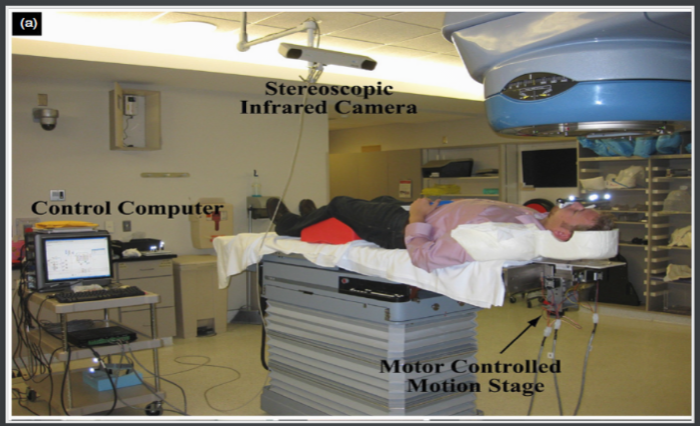
\includegraphics[width=\columnwidth]{figures/igrt.png}
\centering \copyright ~\cite{Wiersma09Dev}
\end{frame}

\begin{frame}
\frametitle{HexaPOD}
\centering 
\includegraphics[width=\columnwidth]{../../../PhDThesis/figures/hexapod.png} \\
\centering Reprinted from \cite{HerrmannHexaPODMPC}
\end{frame}

\begin{frame}
\frametitle{Cyberknife/Novalis systems}
\begin{columns}[c]
	\begin{column}{0.5\textwidth}
		\centering				
		\includegraphics[width=\linewidth]{../../../BOO/figures/cyberknife.jpg}
	\end{column}
	%
	\begin{column}{0.5\textwidth}
		\centering				
		\includegraphics[width=\linewidth]{../../../BOO/figures/cyberknife_rotating.jpg}
%		\includegraphics[width=\linewidth]{../../../Proposal/figures/novalis.png}
	\end{column}
\end{columns}
\end{frame}
%
\begin{frame}
\frametitle{The Novalis ExacTrac Module}
\centering %The Novalis ExacTrac Module
\includegraphics[width=\columnwidth]{../../../Proposal/figures/novalis.png}
\centering \copyright Novalis
\end{frame}

\frame{
	\frametitle{The Case for Soft Robots}
	\begin{itemize}
		\item Frame-based immobilization 
		%
		\vspace{0.1in}
		%
		\begin{itemize}
			\item LINAC misalignments $\implies$ negative dosimetry effects %[\cite{soft_robot:c2}]
			%
			\vspace{0.1in}
			%
			\item $\times$ Fractionated treatments
			%
			\vspace{0.1in}
			%
		\end{itemize}
		\item Frameless RT
		\begin{itemize}
			\item Incompatible with most conventional LINACs 
		\end{itemize}
		%
		\vspace{0.1in}
		%
		\item Cyberknife/Novalis Systems
		%
		\vspace{0.1in}
		%
		\begin{itemize}
			\item Reliance on pre-treatment images
			%
			\vspace{0.1in}
			%
			\item Rigid motion compensation issues
		\end{itemize}
	\item Involuntary patient motion requires adaptive positioning 
	\end{itemize}
\footnotetext{\tiny Morphological computation, Cephalopods, Adaptive Controller for changing head dynamics: shape, weight etc}
}

\subsection{BOO}
\begin{frame}
	\frametitle{Beam Orientation Optimization}
	\begin{itemize}
		\item During treatment planning, a \textbf{b}eam \textbf{o}rientation \textbf{o}ptimization problem (BOO) is  separately solved
		%
		\vspace{0.1in}
		%
		\item Radiation is delivered from
		$\approx(5 − 15)$ different beam orientations during IMRT
		%
		\vspace{0.1in}
		%
		\item BOO determines the best beam angle combinations for delivering radiation
		%
		\vspace{0.1in}
		%
		\item Process of determining beamlets' intensities is termed \textbf{fluence map optimization} (FMO)
	\end{itemize}
\end{frame}
\section{Immobilization}
\begin{frame}
\subsubsection{Experiment Setup}
\frametitle{Vision-based 1-DOF Control}
\begin{columns}[c]
	\begin{column}{0.6\textwidth}
		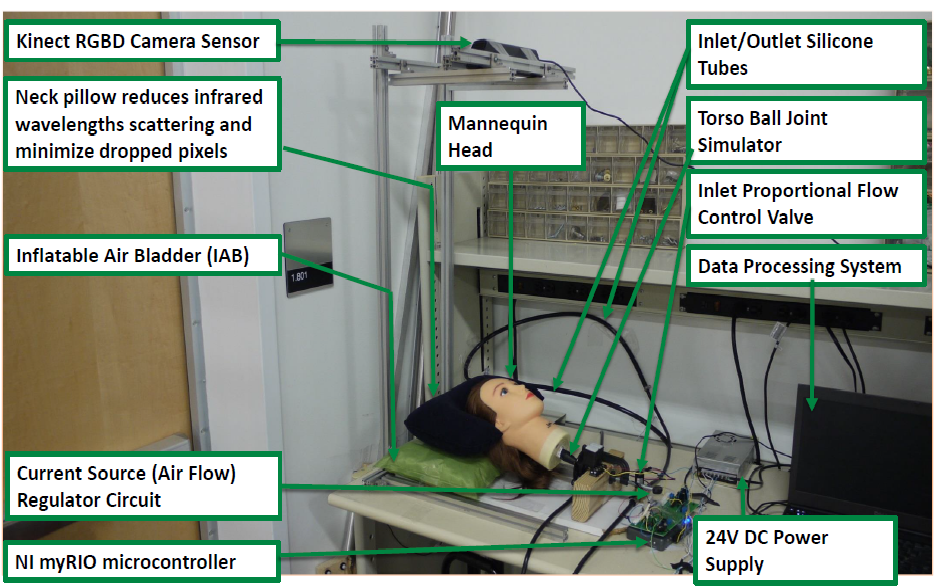
\includegraphics[width=\linewidth,height=.8\linewidth]{figures/setup_1dof.png}
	\end{column}
	%
	\begin{column}{0.48\linewidth}
		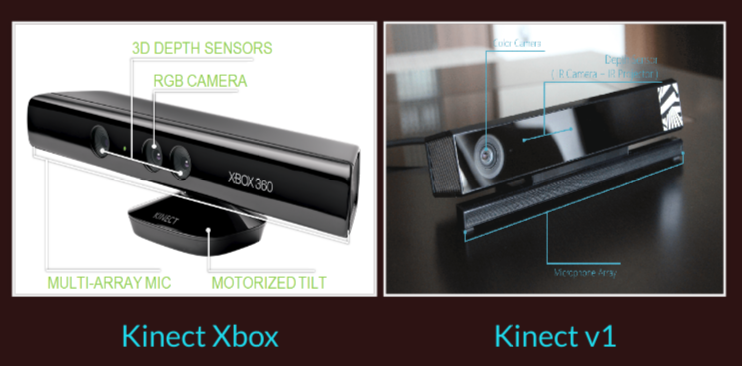
\includegraphics[width=\linewidth]{figures/kinects.png}
	\end{column}
\end{columns}
\end{frame}
%

\begin{frame}
\frametitle{Sensors' Noise Floor}
		\includegraphics[width=\columnwidth]{../../../SoftRobot/CASE2016/Charts/RawDepths.eps}
		%\centering Case for Sensed Observation Filtering
\end{frame}

\begin{frame}
\frametitle{Kalman Filter Model}
		\begin{align}
				\textbf{x}(k) &= \textbf{F}(k)\textbf{x}({k-1})+\textbf{B}(k)\textbf{u}_k+\textbf{G}_k\textbf{w}_k \nonumber \\
				%				
				\vspace{0.1in}
				%
				{z}_s &= \textbf{H}_s(k)\textbf{x}(k)+{v}_s(k) \qquad \qquad s = 1,2 \nonumber \\
				%				
				\vspace{0.1in}
				%
				\textbf{F} &= \begin{bmatrix}
									1 & \Delta T \\
									0	& 1
								\end{bmatrix}; \,
		 a_k \sim \mc{N}(0,  \sigma_a); \, \textbf{G}_k = \textbf{I}_{2x2};  \nonumber \\
		 \textbf{w}(k) &\sim \mathcal{N}(0, \textbf{Q}(k)), \,\,
		\textbf{W}(k) = \left(\begin{array}{c}
		\frac{{\Delta T}^2}{2} \\ \Delta T
		\end{array}\right) \nonumber \\
		%				
		\vspace{0.1in}
		%
		\textbf{Q} &= \textbf{W}\textbf{W}^T{\sigma_a}^2
		= \begin{bmatrix}
		\dfrac{{\Delta T}^4}{4} &	\dfrac{{\Delta T}^3}{2} \\
		\dfrac{{\Delta T}^3}{2} & {\Delta T}^2
		\end{bmatrix}{\sigma_a}^2.
		\end{align}
\end{frame}

\begin{frame}
	\frametitle{State Estimates | Global Fusion of Local Tracks}
	\begin{itemize}
		%\tiny
		\item \textbf{Prediction:}
		\begin{align}
		\hat{\textbf{x}}_{k|k-1}&=\textbf{F}\hat{\textbf{x}}_{k-1|k-1} + \textbf{B}_k\textbf{u}_k  \nonumber \\ 
		\textbf{P}_{k|k-1}&=\textbf{F}_k\textbf{P}_{k-1|k-1}{\textbf{F}_k}^T + \textbf{Q}_k
		\end{align}
		%
		\item \textbf{Update:}
		\small
		\begin{align} 
		\textbf{K}(k) &=  \textbf{P}(k|k-1){ \textbf{H}(k)}^T{[ \textbf{H}(k) \textbf{P}(k|k-1){ \textbf{H}(k)}^T+ \textbf{R}(k)]}^{-1}
		\nonumber \\ 
		\hat{ \textbf{x}}(k|k) &=\hat{ \textbf{x}}(k|k-1) +  \textbf{K}(k) ( \textbf{z}(k) -  \textbf{H}(k) \hat{ \textbf{x}}(k|k-1)) %\tilde{y}_k  
		\nonumber \\ 
		\textbf{P}(k|k)&=( \textbf{I} -  \textbf{K}(k) \textbf{H}(k)) \textbf{P}(k|k-1)
		\end{align}	
		%
%		\item \textbf{Fusion:}
%		\begin{align}
%		\hat{\textbf{x}}(F)(k|k) &= \textbf{P}(F)(k|k)\sum\limits_{s=1}^{N}\left[{\textbf{P}(s)}^{-1}(k|k)\hat{\textbf{x}}(s)(k|k)\right] \nonumber \\
%		\text{where    } \textbf{P}(F)(k|k) &= \left[\sum\limits_{s=1}^{N} {\textbf{P}(s)}^{-1}(k|k)\right]^{-1}. \nonumber
%		\end{align}
	\end{itemize}
\end{frame}

\begin{frame}
	\frametitle{Filtering Results}
		\centering
		\includegraphics[width=.45\columnwidth, height=0.4\columnwidth]{../../../SoftRobot/CASE2016/Charts/KFXbox.eps}
		\includegraphics[ width=.45\columnwidth,height=0.4\columnwidth]{../../../SoftRobot/CASE2016/Charts/Kinect2KF.eps} \\
		 Xbox vs. Kinect v1
		%
		\begin{itemize}
			\small \item 	\textbf{Fusion:}
			\begin{align}
			\hat{\textbf{x}}(F)(k|k) &= \textbf{P}(F)(k|k)\sum\limits_{s=1}^{N}\left[{\textbf{P}(s)}^{-1}(k|k)\hat{\textbf{x}}(s)(k|k)\right] \nonumber %\\
%			\text{where    } \textbf{P}(F)(k|k) &= \left[\sum\limits_{s=1}^{N} {\textbf{P}(s)}^{-1}(k|k)\right]^{-1}. \nonumber
			\end{align}
		\end{itemize}
\end{frame}

\begin{frame}
\frametitle{Fusion Results}
	\centering
\includegraphics[width=\columnwidth]{../../../SoftRobot/CASE2016/Charts/fusion2.eps}
\small Fusion of local state estimates.
\end{frame}

\subsection{Identification}
\begin{frame}
	\frametitle{System Model and LQG Control}
	\begin{itemize}
		\item Obtain optimal model parameters from I/O data through, 
		\begin{align}
		G(t)= \arg \min_{\theta} \, {V_N(\theta, \phi_N)} \label{eq:ident1} 
		\end{align}
		%
		\item From \eqref{eq:ident1}, we obtained
		%
		\begin{align} \label{eq:statemodel} 	
		\textbf{x}(k+Ts) = \textbf{A} \textbf{x}(k) + \textbf{B} \textbf{u}(k) + \textbf{K} \textbf{e}(k) \nonumber \\
		\textbf{y}(k) = \textbf{C} \textbf{x}(k) + \textbf{D} \textbf{u}(k) + \textbf{e}(k)
		\end{align} 
		%			
		\item LQG cost:
		\begin{equation}  \label{eqn:LQ-cost}
		J = \sum\limits_{k=0}^{\mathcal{K}} x^T(k)\,Q\,x(k) +  u(k)^T \, R \, u(k) + 2 x(k)^T \, N \, u(k) \nonumber
		\end{equation}  
		\item Find $u$ from $\Delta u  = \text{arg } \underset{\Delta u}{\text{min }}J $
		%\item  $\Delta{u}$ is a future control sequence
	\end{itemize}
\end{frame}

%\begin{frame}
%	\frametitle{Closed-loop control (Full state observer).}
%		\centering
%	\begin{tikzpicture}[thick,scale=0.4, every node/.style={transform shape}]
%	\sbEntree{E}
%	\sbBloc[4]{bloc1}{$\textbf{B}(k)$}{E}
%	\sbRelier[$\textbf{u}(k)$]{E}{bloc1}
%	\sbBloc[-2.7]{controller}{$\textbf{K}_{opt}$}{E}
%	
%	\sbSortie[-8]{starto}{controller}
%	\sbRelier{starto}{controller}
%	\sbNomLien[0.8]{starto-controller}{$\hat{\textbf{y}}(k)$}
%	
%	\sbCompSum[5]{sumbloc}{bloc1}{+}{+}{+}{}
%	\sbRelier{bloc1}{sumbloc}
%	\sbBloc[4]{integral}{$\int$}{sumbloc}	
%	\sbRelier{sumbloc}{integral}
%	\sbBloc[4]{Hprime}{$C(k)$}{integral}
%	\sbRelier[$x(k)$]{integral}{Hprime}
%	\sbCompSum[4]{sumtwobloc}{Hprime}{+}{}{+}{}
%	\sbRelier{Hprime}{sumtwobloc}
%	\sbDecaleNoeudy[-4]{sumbloc}{u}
%	\sbDecaleNoeudy{integral}{v}
%	\sbBlocr{F}{$A(k)$}{v}
%	\sbRelieryx{integral-Hprime}{F}
%	\sbRelierxy{F}{sumbloc}
%	\sbRelier{u}{sumbloc}   	
%	\sbNomLien[0.5]{u}{$w(k)$}
%	
%	\sbSortie[4]{y}{sumtwobloc}
%	\sbRelier{sumtwobloc}{y}
%	\sbNomLien[0.8]{y}{$y(k)$}
%	
%	\sbDecaleNoeudy[-4]{sumtwobloc}{w}	
%	\sbRelier{w}{sumtwobloc}
%	\sbNomLien[0.5]{w}{$v(k)$}
%	
%	\sbDecaleNoeudy{sumtwobloc-y}{v2}
%	\sbCompSum[8]{sum3bloc}{v2}{-}{+}{}{}
%	\sbRelierxy{y}{sum3bloc}
%	% % Estimator circuit
%	\sbDecaleNoeudy[9]{bloc1}{Ge}
%	\sbDecaleNoeudy[9.5]{Ge}{Gee}
%	\sbBlocr[-2]{Ghat}{$B(k)$}{Gee}
%	
%	\sbSortie[2]{GhatGee}{E}
%	\sbRelieryx{GhatGee}{Ghat}
%	
%	%\sbRelierxy{E}{Ghat}
%	\sbCompSum[7]{sume1}{Ghat}{+}{+}{+}{}
%	\sbRelier{Ghat}{sume1}
%	\sbBloc[4]{integrale}{$\int$}{sume1}	
%	\sbRelier{sume1}{integrale}
%	\sbBloc[4]{Hprimee}{$C(k)$}{integrale}
%	\sbRelier{integrale}{Hprimee}
%	%	\sbNomLien[3]{Hprimee}{$\hat{y}(k)$}
%	
%	\sbRelierxy[$\hat{y}(k)$]{Hprimee}{sum3bloc}
%	\sbDecaleNoeudy[-4]{sume1}{ue}
%	\sbDecaleNoeudy{integrale}{ve}
%	\sbBlocr{Fe}{$A(k)$}{ve}
%	\sbRelieryx{integrale-Hprimee}{Fe}
%	\sbRelierxy{Fe}{sume1}	
%	%  	\sbNomLien[0.5]{u}{$v(k)$}
%	\sbDecaleNoeudy[9]{sum3bloc}{xe}
%	\sbDecaleNoeudy[11]{xe}{xee}
%	
%	\sbDecaleNoeudy[-5.8]{sume1}{Ke}
%	\sbBloc[-1.5]{sume1}{-$K_{obs}$}{Ke}
%	\sbDecaleNoeudy{Ke}{sumpt}
%	\sbRelier{sume1}{sumpt}
%	
%	\sbSortie[-10]{arr}{sum3bloc}
%	\sbRelier[$\epsilon = \hat{y}(k) - y(k)$]{sum3bloc}{arr}  	
%	%\sbLien{sum3bloc}{arr} 
%	\sbDecaleNoeudy[9.5]{sumbloc-integral}{wL}
%	\sbSortie[-0.5]{wLL}{wL}	
%	\sbRelieryx{arr}{wLL}    
%	\sbSortie[-1.5]{Ltop}{sume1}
%	\sbDecaleNoeudy[-1.2]{Ltop}{Ltopey}
%	\sbRelier{wLL}{Ltopey}
%	%\sbNomLien[0.5]{w}{$w(k)$}
%	
%	\sbSortie[3]{we}{integrale} 
%	\sbRelieryx{we}{xee}
%	\sbNomLien[1]{xee}{$\hat{x}(k)$}
%	%\frame{
%	\frametitle{Control Design Goals}
%	\begin{columns}[c]
%		\begin{column}{\textwidth}
%			\begin{itemize}
%				\begin{itemize}
%					\item changing head shapes, size and other anatomic/tumor variations
%				\end{itemize}	
%			\end{itemize}
%		\centering
%		\includegraphics[width=0.95\linewidth,right]{../../IROS2017/Google/figures/mras.jpg}
%		\footnotesize Indirect MRAC system. \tiny (Source mdpi.com)
%			%
%		\end{column}
%		%
%	\end{columns}
%}
%	\sbDecaleNoeudy[3]{xee}{xeebutt}
%	\sbRelier{xee}{xeebutt}
%	\sbDecaleNoeudy[4.2]{Fe}{Ae}
%	\sbBlocr{ngtv}{$-1$}{Ae}
%	\sbRelier{xeebutt}{ngtv}
%	\sbRelierxy{ngtv}{controller}
%	
%	%\sbRelierxy{xee}{controller}
%	%
%	\sbSortie[4]{y}{sumtwobloc}
%	\sbRelier{sumtwobloc}{y}
%	\sbNomLien[0.8]{y}{$y(k)$}    
%	\end{tikzpicture} \\
%	%\centering \small Full Linear Quadratic Gaussian Plant Estimator \\
%	%\small State estimate: 
%	\small $\hat{x}(k+1) = A(k)\hat{x}(k) - K_{obs}[C(k)\hat{x}(k)- y(k)] + B(k)u(k).$
%\end{frame}

\begin{frame}
	\frametitle{1-DOF Control Results}
	%
	\centering
	\includegraphics[width=\columnwidth]{../../../SoftRobot/CASE2016/Charts/LQGI.eps}
%	\includegraphics[width=0.45\columnwidth, height=0.4\columnwidth]{../../../SoftRobot/CASE2016/Charts/LQGIII.eps}
	\\
	\centering LQG Controller on mannequine head.
\end{frame}


\subsection{3-DOF Control}

\begin{frame}
\frametitle{Vision-based 3-DOF Control}
	\centering
	\includegraphics[width=\columnwidth]{../../../SoftRobot/IROS2017/figures/setup/testbed.jpg}
	\centering Hardware Description
\end{frame}
\frame{
	\frametitle{Point Cloud Pre-Processing}
	\begin{columns}[c]
		\begin{column}{0.95\textwidth}	
			\begin{figure}
				\begin{center}
					\includegraphics[width=.8\linewidth]{../../../SoftRobot/IROS2017/figures/seg_cloud_nice.jpg}			
				\end{center}
			\end{figure}
		\end{column}
		%
	\end{columns}
}

\frame{
	\frametitle{Head Pose Estimation}
	\begin{itemize}
		\item Set cloud's centroid as measured point set $\textbf{P} = \{\overrightarrow{p}_i\}$
		%
		\vspace{0.1in}
		%
		\item Get covariance matrix $\Sigma_{px}$ of measured and model point sets: $\textbf{P}$ and $\textbf{X}$
		%
		\vspace{0.1in}
		%
		\item Set cyclic components of anti-symmetric matrix as $\Delta$
		%
		\vspace{0.1in}
		%
		\item Set $\textbf{Q}(\bm{\Sigma}_{px}) = \begin{bmatrix}
		\textbf{tr}(\bm{\Sigma}_{px}) & \bm{\Delta}^T \\
		\bm{\Delta} & \bm{\Sigma}_{px} + \bm{\Sigma}_{px}^T - \textbf{tr}(\bm{\Sigma}_{px})\textbf{I}_3
		\end{bmatrix}$
		%
		\vspace{0.1in}
		%
		\item $q_R = \underset{\text{eig}}{\max} \left(\textbf{Q}(\bm{\Sigma}_{px})\right)$; $q_T = \mu_x - \textbf{R}(q_R)\mu_p$
		%
		\vspace{0.1in}
		%
		\item 	$x_h = (q_T, q_R)$ %Relative orientation and position of head and neck system \wrt table frame	
	\end{itemize}
}

\subsection{Adaptive NeuroControl}
\frame{
	\frametitle{Model Reference Adaptive Control}
	\begin{itemize}
		%
		\item Head and IAB System Model
		%
		\begin{align}
			\dot{\textbf{y}} = \textbf{A}\textbf{y} + \textbf{B} {\bm \Lambda} \left(\textbf{u} - f(\textbf{y}, \textbf{u}) \right) + \textbf{w}(k) \nonumber
		\end{align}
		 %
		 \item  Realize $f(\textbf{\textbf{y}, \textbf{u}})$ with an RNN $\equiv \Theta^T \Phi(\textbf{y})$ 
		 %
		 \vspace{0.1in}
		 %		
		 \item In a ball $\textbf{B}_R \subset D$ %where the domain $D$ in $\reline^n$ contains $f(\cdot)$:
		 %
		 \vspace{0.1in}
		 %		
		 \begin{itemize}
		 	\footnotesize \item an ideal neural network (NN) approximation $f(\cdot): \reline^n \rightarrow \reline^m$, can be realized to a sufficient degree of accuracy, $\varepsilon_f > 0$;
		 \end{itemize}
		 %
 		\vspace{0.1in}
		%				 
		 \item Outside $\textbf{B}_R$:
		 %
		 \vspace{0.1in}
		 %				 
		 \begin{itemize}
		 	\footnotesize \item %the NN approximation error is upper-bounded by a known scalar function $\varepsilon_{max}(\textbf{y})$ \ie
		 	 $\|\varepsilon(\textbf{y})\| \le k_{\text{max}}(\textbf{y}), \quad \, \forall \quad \textbf{y} \in \textbf{B}_R$;
		 \end{itemize}
	\end{itemize}		
}

\frame{
	\frametitle{Adaptive Neuro-Control Scheme}
	\begin{itemize}
		\item Choose $\dot{\textbf{y}}_m = \textbf{A}_m y_m + \textbf{B}_m \textbf{r}$ 
		%
		\vspace{0.1in}
		%
		\item Knowns: $B_m$ and an Hurwitz $A_m$%Adaptive adjustment mechanism from Lyapunov analysis (Parks, P., 1966)
		%
		\vspace{0.1in}
		%				
		\item $\textbf{u} = \underbrace{\hat{\textbf{K}}_y^{\textbf{T}}\textbf{y}}_{\text{state feedback}} + \underbrace{\hat{\textbf{K}}_r^{\textbf{T}} \textbf{r}}_{\text{optimal regulator}} + \underbrace{\hat{f}(\textbf{y, u})}_{\text{approximator}}$
		%
		\vspace{0.1in}
		%
		\item $\hat{\textbf{K}}_y \, \text{ and } \hat{\textbf{K}}_r$ are adaptive gains to be  designed. 
		NB:  $\tilde{\textbf{K}}_x = \textbf{K}_x - \hat{\textbf{K}}_x$
		%	
		\vspace{0.1in}
		%	
		\item Assume ideal model matching conditions $\hat{\textbf{K}}_y = \textbf{K}_y , \, \text{ and } \hat{\textbf{K}}_r = \textbf{K}_r$ 
	\end{itemize}
}

\frame{
	\frametitle{Lyapunov Analysis}
	%
	\begin{itemize}
		\small
		\item \textbf{Theorem:} Given correct choice of adaptive gains $\hat{\textbf{K}}_y$ and $\hat{\textbf{K}}_r$, the error state vector, $\textbf{e}(k)$ with closed loop time derivative $\dot{\textbf{e}}$, is \textit{\textbf{uniformly ultimately bounded}}, and the state $\textbf{y}$ will converge to a neighborhood of $\textbf{r}$ (proof in ~\cite[\S V.A]{Ogunmolu17IROS}).
		%
		\vspace{0.1in}
		%
		
		\item Choose 
					\begin{align}
					\textbf{V}(\textbf{e}, \tilde{\textbf{K}}_y, \tilde{\textbf{K}}_r^T) =
					%
					\textbf{e}^T\textbf{P}\textbf{e} 
					%
					+\textbf{tr}(\tilde{\textbf{K}}_y^T  \bm \Gamma_y ^{-1}  \tilde{\textbf{K}}_y^T |\bm \Lambda|) %\nonumber 
					+\textbf{tr}(\tilde{\textbf{K}}_r^T \Gamma_r^{-1} \tilde{\textbf{K}}_r |\bm \Lambda|) \nonumber
					\end{align}
		%
		\item Neural network model $\hat{f}(\textbf{y}) = \hat{{\bm \Theta}}^T {\bm \Phi}(\textbf{y}) + \bm \varepsilon_f(\textbf{y})$
	\end{itemize}
}

\frame{
	\frametitle{Proof Main Matter}
	%\begin{itemize}		
		%
		\begin{align}
		\lyapder(\textbf{e}, \tilde{\textbf{K}}_y, \tilde{\textbf{K}}_r^T) &= -\textbf{e}^T\textbf{Qe}  -2 \textbf{e}^T\textbf{PB}\lamb \neterror \nonumber \\
		\lyapder(\textbf{e}, \tilde{\textbf{K}}_y, \tilde{\textbf{K}}_r^T) & \le -\lambda_{low}\|\textbf{e}\|^2 + 2\|\xbold{e}\| \|\textbf{PB}\|\lambda_{high}(\lamb) \bm{\varepsilon}_{max} \nonumber 
		\end{align}
		
		\begin{tcolorbox}[title=Term Contributions,colframe=green!35!blue!75]
			\begin{itemize}
				\item  $\hat{\textbf{K}}_y^{\textbf{T}}\textbf{y} $  keeps  $\textbf{y} \in \textbf{B}_R$ stable; $\hat{\textbf{K}}_r^{\textbf{T}} \textbf{r}$ reference tracking
				%
				\item $\hat{f}(\textbf{y}, \control)$ ensures states starting outside  set $\textbf{y} \in \textbf{B}_R$ converge to $\textbf{B}_R$ in finite time 
			\end{itemize}
		\end{tcolorbox}	
	%\end{itemize}
}

\frame{
	\frametitle{Proof Main Matter}
	%
	\begin{itemize}
		\item $\lambda_{low}, \lambda_{high}$ $\equiv$ minimum and maximum characteristic roots of $Q \text{ and }\lamb$ respectively
		%
		\vspace{0.1in}
		%
		\item $\dot{\xbold{V}}(\cdot)$ is thus negative definite outside the compact set:
		%
		\vspace{0.1in}
		%
		\begin{itemize}
			\item $\chi =\left(\textbf{e}: \|\textbf{e}\| \le \frac{2\|\textbf{PB}\|\lambda_{high}(\bm \Lambda)\varepsilon_{max}(\textbf{y})}{\lambda_{low}(\textbf{Q})}\right)$
		\end{itemize}
		%
		\vspace{0.1in}
		%
		\item Therefore, the error $\textbf{e}$ is uniformly ultimately bounded $\textbf{y}(t) \rightarrow 0$ as $t \rightarrow \infty$
	\end{itemize}
}
\frame{
	\frametitle{Results}
	\begin{itemize}
				\item Choose
				\begin{align}
				\textbf{P} = 
				\begin{bmatrix}
				-\frac{170500}{2668} & 0 & 0 \\
				0 & -\frac{170500}{2668} & 0 \\
				0 & 0 & -\frac{170500}{2668}
				\end{bmatrix} \nonumber
				\end{align}			
				\item and set 	
				\begin{align}
					\textbf{B} = 
					\begin{bmatrix}
					1 &\, 1 &\, 0 &\, 0  &\, 0 &\, 0 \\
					0 &\,  0 &\, 1 &\, 1 &\, 0 &\, 0 \\
					0 &\,  0 &\, 0 &\, 0 &\,  1 &\, 1 
					\end{bmatrix} \nonumber
					\end{align}
			\end{itemize}
}

\frame{
	\frametitle{Results}
	%
		\centering
		\includegraphics[width=0.45\columnwidth,height=0.35\columnwidth]{../../IROS2017/Google/figures/expt2a.eps}
		\includegraphics[width=0.45\columnwidth,height=0.35\columnwidth]{../../IROS2017/Google/figures/roll_nice.eps}
		\footnotesize \centering 
		[Left]: Goal command: $\left(z, \theta, \phi\right)=\left(2.5mm, 0.25^\circ, 35^\circ\right)$ to $\left(14mm, 1.6^\circ, 45^\circ\right)^T$. 
		\centering[Right]: Head roll tracking.
}

\section{Deformation}
\begin{frame}
\frametitle{Model of a 6-DOF SoRo Mechanism}
\centering
Page left blank intentionally.
\end{frame}

\begin{frame}
\frametitle{Existing Modeling Approaches}
\begin{itemize}
	\tiny
	\item Finite element modeling:~\cite{Nesme2005, Nesme2006, JamesBern, GentBook}
	%
	\vspace{0.1in}
	%
	\item Constant curvature approaches:~\cite{Hannan2003, Hannan2000, Jones2006} 
	%
	\vspace{0.1in}
	%
	\item Piecewise constant curvature model:~\cite{Jones2006}
	%
	\vspace{0.1in}
	%
	\item Cosserat brothers' beam theory:~\cite{Renda2014Cosserat, TrivediCosserat}
	%
	\item Non-constant curvature approaches
	%
	\vspace{0.1in}
	%
	\begin{itemize}
		\tiny
		\item Continuum approximation of hyper-redundant sytems \eg~\cite{HyperMochi, Chirikjian1995, Chirikjian1994}, 
		%
		\vspace{0.1in}
		%
		\item Spring-mass models for semi-rigid robots:~\cite{yekutieli2005dynamic, zheng2012dynamic}, 
		%
		\vspace{0.1in}
		%
		\item Geometric continuum models:~\cite{boyer2006macro, GentBook, OgdenBook, SedalFREE2018, Holzapfel2000, rucker2010geometrically, Demirkoparan}
	\end{itemize}
\end{itemize}
\end{frame}

\begin{frame}
\frametitle{A Continuum Mechanics Model for IAB Deformation}
\begin{itemize}
	\item \textbf{Context}: Model-based approaches generally give better material responses
	%
	\vspace{0.1in}
	%
	\item \textbf{Contributions}
	
	\begin{itemize}
		\item Finite elastic (geometric continuum)  model for IAB deformation
		%
		\vspace{0.1in}
		%
		\item Component stresses, internal pressurization, and particle positions/velocities
		%
		\vspace{0.1in}
		%
		\item Synthesis of IAB contact velocities and head motion: manipulation dynamics, selection maps, and contact forces
	\end{itemize}
\end{itemize}
\end{frame}

\begin{frame}
\frametitle{IAB Kinematics}
\centering 
	\begin{columns}[c]
	\begin{column}{.5\textwidth}
		\includegraphics[width=0.9\linewidth]{../../../PhDThesis/figures/head_on_4iab.png}
	\end{column}
	%	
	\begin{column}{.5\textwidth}
		\-
		\hspace{0.25em}
		\includegraphics[width=0.9\linewidth]{../../../PhDThesis/figures/IAB_Head.png}
	\end{column}
\end{columns}
\end{frame}

\begin{frame}
	\frametitle{Fibers and deformation}
	\begin{itemize}
		\item  The rate of deformation from a  configuration $\mc{B}_0$ to a current configuration $\mc{B}$ in component form
		%
		\begin{align}
		\text{dx}_i &= \dfrac{\partial x_i}{\partial X_\alpha} \text{dX}_\alpha,
		\text{  with invariant form }
		\textbf{dx} = \textbf{FdX} \nonumber \\ %\text{ or } \deformationgrad = \bm{\nabla} \otimes \currconf(\textbf{X})
		&\text{
			for an observer \textbf{O} in \eg basis }\{E_\alpha\} \nonumber
		\end{align}
		%
		\item A \textit{material line element} (a fiber) $\textbf{dX}$ at a point \textbf{X}  are  particles lying along $\fiber$ at a point $\textbf{X}$ of a soft body
		%
		\vspace{0.1in}
		%
		\item $\fiber \neq 0 \implies \deformationgrad \fiber \neq 0$ for all  $\fiber \neq 0$. Therefore, $\deformationgrad$ 		must be a non-singular 	tensor, imposing the restriction, $\text{ det }\deformationgrad \neq 0$
	\end{itemize}
\end{frame}

%\begin{frame}
%	\frametitle{Isochoricity and Incompressibility}
%	\begin{itemize}
%		\item If the volume does not change locally during deformation at \textbf{X}, then
%		\begin{align}
%		J \equiv \text{det } \deformationgrad = 1
%		\label{eq:isochoric}
%		\end{align} 
%		%			
%		\item Permanent isochoricity and incompressibility constraints
%		%
%		\begin{align}
%			C(\deformationgrad) \equiv \text{det } \deformationgrad - 1 = 0 
%		\end{align}
%	\end{itemize}
%\end{frame}

\begin{frame}
	\frametitle{Deformation Analysis of a Soft Continuum Robot}
	\begin{figure}[!tb]
		\centering
		\begin{minipage}[b]{0.45\textwidth}
			\includegraphics[width=\textwidth]{../../../PhDThesis/figures/spherical_coords_ref.png}
			%\small $R_i \le R \le R_o, \quad 0 \le \Theta \le 2\pi, \quad 0 \le \Phi \le \pi$
		\end{minipage}
		\hfill
		\begin{minipage}[b]{0.50\textwidth}
			\includegraphics[scale=0.4, width=\textwidth]{../../../PhDThesis/figures/spherical_coords.png}
		\end{minipage}
		%{Deformation in spherical polar coordinates.}
		\label{fig:spherical_coords}
	\end{figure}
	%
	with
	%
	\begin{align}
	R_i \le R \le R_o, \, 0 \le \Theta \le 2\pi, \, 0 \le \Phi \le \pi  \nonumber \\
 	r_i \le r \le r_o, \, 0 \le \theta \le 2\pi,  \, 0 \le \phi \le \pi
	\label{eq:polar_coordinates_ref}
	\end{align}
\end{frame}


\begin{frame}
\frametitle{Deformation Analysis}
%
\begin{figure}[!tb]
	\centering
	\begin{minipage}[b]{0.45\textwidth}
		\includegraphics[width=\textwidth]{../../../PhDThesis/figures/deformation_ref.png}
		%\caption{Spherical Polar Coordinates in Reference Configuration.}
	\end{minipage}
	\hfill
	\begin{minipage}[b]{0.5\textwidth}
		\includegraphics[width=\textwidth]{../../../PhDThesis/figures/deformation_curr.png}
	\end{minipage}
	%{Radii change under deformation with preservation of radial symmetry}
	\label{fig:radii_change}
\end{figure}
%
\begin{itemize}
	\item  An isochoric homogeneous deformation implies
\end{itemize}
%
\begin{align}
\dfrac{4}{3}\pi\left(R^3 - R_i^3\right) &= \dfrac{4}{3}\pi\left(r^3 - r_i^3\right),\,\theta = \Theta \,\, \phi = \Phi \nonumber \\
	 r^3 &= R^3 + r_i^3 - R_i^3, \,\, \theta = \Theta, \,\, \phi = \Phi
\label{eq:spherical_transformation}
\end{align}
\end{frame}

\begin{frame}
\frametitle{Stored Energy Invariants and Principal Ratios}
\begin{itemize}
	\item Spherically symmetric deformation implies coincidence of the \textit{Lagrangean} and \textit{Eulerian} axes 
	%
	\vspace{0.1in}
	%
	\item Thus, principal ratios  along azimuthal and zenith axes is $\lambda_\theta = \lambda_\phi = r/R$
	%
	\vspace{0.1in}
	%
	\item We have $\lambda_r\lambda_\phi\lambda_\theta=1$ from the incompressibility of the IAB material. Thus, $\lambda_r = \frac{R^2}{r^2}$ so that 
	%\begin{tcolorbox}[title=Stored Energy Invariants (Mooney Form)]
	\begin{align}
	I_1 = \lambda_r^2 + \lambda_\phi^2 + \lambda_\theta^2, \, \text{ and } \, I_2 =  \lambda_r^{-2} + \lambda_\phi^{-2} + \lambda_\theta^{-2}.
	\label{eq:invariants}
	\end{align}
	%\end{tcolorbox}
	%
\end{itemize} 
%
\end{frame}

\begin{frame}
	\frametitle{Strain Tensor and Deformation Gradient}
	%
	\begin{itemize}
		\item Mooney-Rivlin strain energy form for small deformations:
		\begin{align}
		\strain = \frac{1}{2}C_1(I_1-3) + \frac{1}{2}C_2(I_2-3).
		\label{eq:Mooney}
		\end{align}
%		\begin{itemize}
%			\item \small \eqref{eq:Mooney} is valid even for large elastic deformations of incompressible and isotropic materials~\cite{Rivlin1950}
%		\end{itemize}
%
\vspace{0.1in}
%
		\item  Deformation gradient in spherical polar coordinates
	\end{itemize}
\begin{align}
\deformationgrad &= \lambda_r \basis_r \otimes \basis_R + \lambda_\phi \basis_\phi \otimes \basis_\Phi + \lambda_\theta \basis_\theta \otimes \basis_\Theta \nonumber \\
%
\deformationgrad &= \frac{R^2}{r^2}  \basis_r \otimes \basis_R + \frac{r}{R} \basis_\phi \otimes \basis_\Phi + \frac{r}{R} \basis_\theta \otimes \basis_\Theta.		
\label{eq:deformation_grad}
\end{align}
%
	\begin{align}
	\leftcauchy   &= \deformationgrad \, \deformationgrad^T &:= \text{Left Cauchy-Green deformation tensor} \nonumber \\ 
	\rightcauchy &= \deformationgrad^T\deformationgrad &:= \text{Right Cauchy-Green deformation tensor}  \nonumber
	\end{align}
\end{frame}

\begin{frame}
	\frametitle{Stress Laws and Constitutive Equations}
	\centering
	\includegraphics[width=.45\columnwidth]{../../../PhDThesis/figures/Fibre.png}
	\includegraphics[width=.5\columnwidth]{../../../PhDThesis/figures/Fibre3d.png}
	\tiny{Stress distribution on the internal continuum's differential surface, $dS$.}
\end{frame}

\begin{frame}
	\frametitle{Invariants of Deformation}
		%
	%\begin{tcolorbox}[title=IAB Invariants]
		\begin{align}
		I_1 &= \trace{\rightcauchy} =  \dfrac{R^4}{r^4} + \dfrac{2 \, r^2}{R^2};  \,
		%
		I_2 = \textbf{tr}\left(\rightcauchy^{-1}\right) = \dfrac{r^4}{R^4} + \dfrac{2 \, R^2}{r^2}.
		\end{align}
		\label{eq:invariants_polar}
	%\end{tcolorbox}
	%
	For a constrained elastic material, we have the following constitutive relation 
	%
\begin{align}
\cauchystress &= \materialresponse(\deformationgrad) + q \deformationgrad \dfrac{\partial \bm{\Lambda}}{\partial \deformationgrad}(\deformationgrad) \nonumber \\
&= \materialresponse(\deformationgrad) - p \deformationgrad \deformationgrad^{-T}  \text{det}(\deformationgrad) \nonumber \\
&= \materialresponse(\deformationgrad) - p \identity %\text{det}(\deformationgrad)
\label{eq:cauchy_stress2}
\end{align}
\end{frame}

\begin{frame}
	\frametitle{Cauchy stress and hydrostatic pressure}
	%
	In terms of the stored strain energy, we have the stress tensor field as
	\begin{align}
	\cauchystress &= \begin{bmatrix}
	\stresscomp_{rr} &  \stresscomp_{r\phi} &  \stresscomp_{r\theta}  \\
	\stresscomp_{\phi r} &   \stresscomp_{\phi \phi}  &   \stresscomp_{\phi \theta}  \\
	\stresscomp_{\theta r} &     \stresscomp_{\theta \phi} &     \stresscomp_{\theta \theta}
	\end{bmatrix} = \dfrac{\partial W}{\partial \deformationgrad} \deformationgrad^T - p\identity, 
	%&= C_1 \leftcauchy - C_2 \rightcauchy^{-2}  - p\identity (\text{ see derivation in thesis.})\nonumber 
	\label{eq:cauchy_stress}
	\end{align}
	%
	or
%	\begin{tcolorbox}[title=Stress-Strain Constitutive Law]
		\begin{align}
		\cauchystress &= C_1 \leftcauchy - C_2 \rightcauchy^{-2} - p \identity
		\label{eq:stress_constitutive}
		\end{align}
	where $C_1, C_2$ are appropriate choices of the IAB material moduli; %so that the normal stress components are 
	%
	\begin{subequations}
		\begin{align}
		\stresscomp_{rr} &= -p + C_1 \dfrac{R^4}{r^4} - C_2 \dfrac{r^8}{R^8} \\
		\stresscomp_{\theta \theta} = \stresscomp_{\phi \phi} &= -p + C_1 \dfrac{r^2}{R^2} - C_2 \dfrac{R^8}{r^8} 
		\end{align}
		\label{eq:stress_compos}
	\end{subequations}
%	\end{tcolorbox}
\end{frame}

\begin{frame}
	\frametitle{Contact-Free BVP for IAB Deformation}
	\begin{itemize}
		\item \small Consider an IAB with boundary conditions,
		%
		\begin{align}
		\stresscomp_{rr}|_{R=R_o} = -P_\text{atm}, \quad \stresscomp_{rr}|_{R=R_i} = -P_\text{atm} - P
		\label{eq:boundary_conds}
		\end{align}
		%
		\item \small{If the stress components, $\stresscomp_{ij}$, satisfy hydrostatic equilibrium,  equilibrium equations for the body force $\bm{b}'s$ physical component vectors, $b_r, b_\theta, b_\phi$ are}
		%
		\begin{subequations}
			\tiny{
			\begin{align}
			-b_r &= \frac{1}{r^2}\frac{\partial}{\partial r}(r^2 \stresscomp_{rr}) + \frac{1}{r \sin\phi}\frac{\partial}{\partial \phi}(\sin \phi \stresscomp_{r \phi}) + \frac{1}{r \sin\phi}\frac{\partial}{\partial \theta}(\stresscomp_{r \theta}) -  \frac{1}{r}(\stresscomp_{\theta\theta}+ \stresscomp_{\phi \phi})
			\label{eq:polar_coord_a}
			\\
			-b_\phi &= \frac{1}{r^3}\frac{\partial}{\partial r}(r^3 \stresscomp_{r\phi}) + \frac{1}{r \sin\phi}\frac{\partial}{\partial \phi}(\sin \phi \stresscomp_{\phi \phi}) + \frac{1}{r \sin\phi}\frac{\partial}{\partial \theta}(\stresscomp_{\theta \phi}) -  \frac{\cot \phi}{r}(\stresscomp_{\theta\theta})
			\label{eq:polar_coord_b}
			\\
			-b_\theta &= \frac{1}{r^3}\frac{\partial}{\partial r}(r^3 \stresscomp_{\theta r}) + \frac{1}{r \sin^2\phi}\frac{\partial}{\partial \phi}(\sin^2 \phi \stresscomp_{\theta \phi}) + \frac{1}{r \sin\phi}\frac{\partial}{\partial \theta}(\stresscomp_{\theta \theta})
			\label{eq:polar_coords_c}
			\end{align}
		}
			\label{eq:polar_coords}
		\end{subequations}
	%
	\item \small Cauchy's 1st law of motion
	\begin{align}
	\text{div } \cauchystress^T  + \rho \textbf{b} = \rho \dot{\textbf{v}}
	\label{eq:cauchy_law1}
	\end{align}
	\end{itemize}
\end{frame}

\begin{frame}
	\frametitle{Stress at Hydrostatic Equilibrium}
	\begin{itemize}
		\item Equilibrium therefore implies that %$\textbf{div } \cauchystress = 0$
		%
		\[
		\textbf{div } \cauchystress = 0
		\]
		%
		\[
		\small
		\frac{1}{r}\frac{\partial}{\partial r}(r^2 \stresscomp_{rr}) = (\stresscomp_{\theta\theta}+ \stresscomp_{\phi \phi})
		\]
		\item Whereupon,
		%
		\begin{align}
		\small
		P  &=  2 C_1\int_{R_i}^{R_\circ} 			\left(\frac{1}{r}-\frac{R^6}{r^{7}}\right)dR+2C_2\int_{R_i}^{R_\circ} \left(\frac{r^{5}}{R^6} - \frac{R^{10}}{r^{11}}\right)  dR \nonumber \\
			&\equiv \int_{r_i}^{r_\circ} \left[2 C_1\left(\frac{r}{R^2}-\frac{R^4}{r^{5}}\right)+2 C_2\left(\frac{r^{7}}{R^8} - \frac{R^{8}}{r^{9}}\right)\right]  dr. %, \quad r_i \le r \le r_\circ
		\label{eq:internal_pressure}
		\end{align}
		%
		\item \eqref{eq:internal_pressure} completely determines the deformation kinematics of the IAB material at rest. 
	\end{itemize}
\end{frame}

\begin{frame}
	\frametitle{Example I: IAB Deformation (Extension)}
	\centering
		\begin{tabular}{@{}c@{}c@{}c@{}}
		\toprule
		& Deformation Parameters & \\
		\midrule
		$C_1=11,000$ &  $C_2 = 22,000$ & $R_i = 10cm, \, r_i = 13cm$ \\
		%
		$R_\circ = 15cm$ & $r_\circ = 16.60cm$ &  $P = 14.52 psi$  
		%
		\\
		\midrule
		\bottomrule
	\end{tabular}
	%
	\centering
	\includegraphics[width=\columnwidth]{../../../PhDThesis/figures/deformation/mesh_1.png}
\centering 
\end{frame}


\begin{frame}
\frametitle{Example I: Deformation (Extension) Results}
	\centering
	\begin{tabular}{@{}c|@{}|c@{}}
		\toprule
		%& Deformation Results & \\
		\midrule 
		Mesh Time: $0.8838$s  & Total Time: $4.7782$s \\
		%
		$\nu=0.45$ & $\rho = 9.8446\times 10^{-4} kG/m^3$ 
		%
		\\
		\midrule
		\bottomrule
	\end{tabular}
\includegraphics[width=\columnwidth]{../../../PhDThesis/figures/deformation/xyz_1.png}
\end{frame}

\begin{frame}
\frametitle{Example II: IAB Deformation (Extension)}
\centering
\begin{tabular}{@{}c@{}c@{}c@{}}
	\toprule
	& Deformation Parameters & \\
	\midrule
	$C_1=500,000$ &  $C_2 = 1,000,000$ & $R_i = 7.5cm, \, r_i = 12cm$ \\
	%
	$R_\circ = 10 cm$ & $r_\circ = 13.21cm$ & $P = 14.5193 psi$  
	%
	\\
	\midrule
	\bottomrule
\end{tabular}
%
\centering
\includegraphics[width=\columnwidth]{../../../PhDThesis/figures/deformation/mesh_1.png}
\centering 
\end{frame}


\begin{frame}
\frametitle{Example II: Deformation Results (Extension)}
\centering
\begin{tabular}{@{}c|@{}|c@{}}
\toprule
%& Deformation Results & \\
\midrule 
Mesh Time: $.9143$s  & Total Time: $4.1445$s \\
%
$\nu=0.4995$ & $\rho = 10^{-4}\,kg/m^3$ 
%
\\
\midrule
\bottomrule
\end{tabular}
\includegraphics[width=\columnwidth]{../../../PhDThesis/figures/deformation/xyz_2.png}
\end{frame}

\begin{frame}
\frametitle{Example III: IAB Deformation (Compression)}
\centering
\begin{tabular}{@{}c@{}c@{}c@{}}
	\toprule
	& Deformation Parameters & \\
	\midrule
	$C_1=500,000$ &  $C_2 = 1,200,000$ & $R_i = 12cm, \, r_i = 10cm$ \\
	%
	$R_\circ = 15 cm$ & $r_\circ = 13.83cm$ & $P = -27.3631 \, \text{psi}$ 
	%
	\\
	\midrule
	\bottomrule
\end{tabular}
%
\centering
\includegraphics[width=\columnwidth]{../../../PhDThesis/figures/deformation/mesh_3.png}
\centering 
\end{frame}


\begin{frame}
\frametitle{Example III: Deformation Results (Compression)}
\centering
\begin{tabular}{@{}c|@{}|c@{}}
\toprule
%& Deformation Results & \\
\midrule 
Mesh Time: $.8625$s  & Total Time: $4.5338$s \\
%
$\nu=0.45$  &  $\rho = 12\times10^{-4}\,kg/m^3$ 
%
\\
\midrule
\bottomrule
\end{tabular}
\includegraphics[width=\columnwidth]{../../../PhDThesis/figures/deformation/xyz_3.png}
\end{frame}

\begin{frame}
\frametitle{Example IV: IAB Deformation (Compression)}
\centering
\begin{tabular}{@{}c@{}c@{}c@{}}
	\toprule
	& Deformation Parameters & \\
	\midrule
	$C_1=1.1e12$ &  $C_2 = 2.2e10$ & $R_i = 10cm, \, r_i = 8cm$ \\
	%
	$R_\circ = 19 cm$ & $r_\circ = 18.54 cm$ & $P = -27.3631 \text{psi}$ 
	%
	\\
	\midrule
	\bottomrule
\end{tabular}
%
\centering
\includegraphics[width=\columnwidth]{../../../PhDThesis/figures/deformation/mesh_4.png}
\centering 
\end{frame}


\begin{frame}
\frametitle{Example IV: Deformation Results (Compression)}
\centering
\begin{tabular}{@{}c|@{}|c@{}}
\toprule
%& Deformation Results & \\
\midrule 
Mesh Time: $0.823576$s  & Total Time: $4.5098$s \\
%
$\nu=0.495$  &  $\rho = 2.0\times 10^{-5} \,kg/m^3$ 
%
\\
\midrule
\bottomrule
\end{tabular}
\includegraphics[width=\columnwidth]{../../../PhDThesis/figures/deformation/xyz_4.png}
\end{frame}
\section{Multi-DOF Kinematics}
\begin{frame}
	\frametitle{Multi-DOF IAB Kinematics \& Dynamics}
%	\centering This page is left blank intentionally.
	\begin{itemize}
		\item \textbf{Outline}
		%
		\begin{itemize}
			\item Solve boundary-value problem for IAB kinematics with head contact
			%
			\vspace{0.1in}
			%
			\item Relate Deformation Kinematics to Contact Dynamics
			%
			\vspace{0.1in}
			%
			\item Derive head velocity and orientation in terms of contact velocities
			%
			\vspace{0.1in}
			%
			\item Derive Newton-Euler's Dynamics of the Head-IAB system for control 
		\end{itemize}
	\end{itemize}
\end{frame}


\begin{frame}
	\frametitle{Contact Kinematics}
	\begin{columns}[c]
		\begin{column}{.45\textwidth}
			\centering
			\begin{itemize}
				\tiny
				%
				\vspace{0.1in}
				%
				\item All friction cones lie within a soft contact type model:~\cite{Nguyen1988}
				%
				\begin{align}
					FC &= \{\contactforcecomp_{c} \in \reline^n: \|f^t_{c_{ij}}\| \le \mu_{ij}\|f_{c_i}^n\|, \nonumber \\
					 i&=1, \ldots,k, \quad j=1,\ldots, m_i  \}
				\end{align}
				%
				\item $f_{c_{ij}}^t = $  tangent component of $j^{th}$ element of contact force
				%
				\vspace{0.1in}
				%
				\item $f_{c_i}^n = $ $i^{th}$ contact's normal force, and $\mu_{ij}$ is $f_{c_{ij}}$'s coefficient of friction
				%
				\vspace{0.1in}
				%
				\item Contact force within friction cone:
				\begin{align}
				\contactforce_{c_i} = \begin{bmatrix}
				\identity & {0}\\
				{0} & \gaussianmap_{c_i}
				\end{bmatrix}
				%
				\begin{bmatrix}
				\contactforcecomp_{c_i} \\ \contacttorquecomp_{c_i}
				\end{bmatrix},
				\label{eq:soft_contact}
				\end{align}
			\end{itemize}
		\end{column}
		\begin{column}{0.65\textwidth}
			\includegraphics[width=.8\linewidth, height=.75\columnwidth]{../../../PhDThesis/figures/Cone_Forces.png}\\
			\tiny \centering IAB-Head Soft Contact
		\end{column}
	\end{columns}
\end{frame}

\begin{frame}
	\frametitle{Contact Map}
	\begin{itemize}
		\item Soft contact type is the map
		%
		\begin{align}
		\manipmap_i(r_{c_i}, \twist_h) = \begin{bmatrix}
		\identity & \bm{0} \\
		{\hat{\omega}}(r_{c_i}) & \identity
		\end{bmatrix} \selmap_i(\twist_h, \twist_r)
		\label{eq:force_constraint}
		\end{align}
		%
		\item Head never rolls out of convex sum of conic forces of individual IABs
		%
		\vspace{0.1in}
		%
		\item For multiple IABs acting on the head, resultant head force is a superposition of individual IAB forces 	
		%
		\begin{align}
		\contactforce_h = \begin{bmatrix}
		\manipmap_1, \ldots, \manipmap_8
		\end{bmatrix}
		%
		\left(\begin{array}{c}
		\contactforce_{c_1} \\ \contactforce_{c_8}
		\end{array}\right) = \manipmap \contactforce_{c},
		\label{eq:head-contact-force}
		\end{align}
		%
		\item where $F_h \in \reline^6$ and $F_c \in \reline^{m_1} \times \reline^{m_2} \times \ldots \times \reline^{m_8}$
	\end{itemize}
\end{frame}

\begin{frame}
	\frametitle{BVP for IAB-Head Dynamics}
	\begin{itemize}
		\item 
		Velocity constraint dual
		\begin{align}
		\left(
		\begin{array}{c}
		\tilde{v}_{c_i} \\ \tilde{\omega}_{c_i}
		\end{array}
		\right) 
		%
		= \begin{bmatrix}
		\identity & \hat{\omega}(r_{c_i}) \\
		0 & \identity
		\end{bmatrix}
		%
		\left(
		\begin{array}{c}
		{v}_{c_h} \\ {\omega}_{c_h}
		\end{array}
		\right).
		\end{align}
		%
		\item If $v_c$ is the conjugate velocity to $f_c$, then forces exerted by the fingers are
		%
		\begin{align}
			\left(
			\begin{array}{c}
				v_c \\ \omega_c
			\end{array}\right) = \manipmap^T \left(\begin{array}{c} v_h \\ \omega_h \end{array}\right)
		\end{align}
		%
		\item Equations of motion for IAB continuum
		\begin{subequations}
			\begin{align}
			\dot{\rho} + \rho \text{div} \textbf{v} &= 0 \label{eq:continuum-1}, \\
			\cauchystress^T &= \cauchystress,  \label{eq:continuum-2}\\
			\text{div} \cauchystress^T + \rho \bm{b} &= \rho \dot{\textbf{v}} \label{eq:continuum-3}
			\end{align} 
		\end{subequations}
	\end{itemize}
\end{frame}

\begin{frame}
	\frametitle{IAB Forces under Entropy}
	\tiny
	Head forces (see derivation in \cite[Appendix C.]{OgunmoluThesis}) are in part the  internal pressurization, $P_i$, and the stress tensor components $\{\stresscomp_{\phi \phi}(\epsilon), \stresscomp_{\theta \theta}(\zeta)\}$, 
	%
	\begin{subequations}
		\tiny
		\begin{align}
		P  &= \int_{r_i}^{r_\circ} \left[\frac{1}{r}\left(
		-2p + 2 C_1 \frac{r^2}{R^2} - 2 C_2 \frac{R^8}{r^8}
		\right) - \rho b_r +  \rho \cos \theta \left(2\dot{r}\dot{\phi}\cos\theta + r \cos\theta \ddot{\phi}-2r\dot{\theta}\dot{\phi}\sin\theta\right) \nonumber \right. \\
		& \left. \quad - \rho \sin\phi\left(\cos\theta (-\ddot{r}+r\dot{\theta}^2 + r\dot{\phi}^2)+\sin\theta(2 \dot{r}\dot{\theta}+r\ddot{\theta})\right) \vphantom{}  \right] dr \label{eq:radial-stress-integ} \\
		%	
		\stresscomp_{\phi \phi}(\epsilon) &= 
		- \int_{\epsilon}^{\pi} \left[ r \rho\left[\cos \phi\left(2 r \dot{\theta} \dot{\phi} \cos \theta +(2 \dot{r} \dot{\phi}+r \ddot{\phi}) \sin \theta\right)+\right.  \right. \nonumber \\ 
		%
		& \quad \left. \left. \sin \theta
		\left(2 \dot{r} \dot{\theta} \cos \theta +r \ddot{\theta} \cos \theta +(\ddot{r}- r\dot{\theta}^{2}-r\dot{\phi}^{2}) \right) \sin \phi  \vphantom{} \right] - \rho r b _\theta \vphantom{} \right]d\phi, \, 0 \le \epsilon \le \pi
		\label{eq:azim-stress-integ} \\
		%
		\stresscomp_{\theta \theta}(\zeta) &= %2 \pi 
		- \int_{\zeta}^{2\pi}	\left[-r \rho b_{\theta}\sin\phi + r  \rho \sin\phi \cos \phi\left(\ddot{r} - r \dot{\phi}^2 \right)  - r  \rho \sin^2\phi \left(2 \dot{r}\dot{\phi} + r \ddot{\phi}\right) \right]d\theta, \,  0 \le \zeta \le 2 \pi %\nonumber \\
		%	& \qquad \qquad 0 \le \zeta \le 2 \pi.
		\label{eq:polar-stress-integ}
		\end{align}
		\label{eq:stress-integ}
	\end{subequations}
	%
	 where $0 \le \epsilon \le \pi, 0 \le \zeta \le 2 \pi$ and  gravity forces. 
\end{frame}

\begin{frame}
	\frametitle{ Piola-Kirchoff Stress Tensor \& Contact Forces}
	%
	\begin{itemize}
		%
		\item For an infinitesimal vector element $\textbf{dA}$ in $\currconfbody_0$,
		we have $\textbf{dA} = \textbf{N} \text{dA}$ for a surface dA with outward normal map \textbf{N}
		%
		\item Similarly, in configuration $\currconfbody$,  $\textbf{da} = \textbf{n}\, \text{da}$ for an outward normal map \textbf{n}
		%
		\item Therefore on the IAB boundary, volume preservation implies that
		%
		\begin{align}
		\int_{\partial \currconfbody} \cauchystress \, \textbf{n} \, \text{da} = \int_{\partial \currconfbody_\circ} J \, \cauchystress \, \deformationgradcur  \, \textbf{N } \text{dA}.
		\end{align}
		%
		\item Define the Piola-Kirchoff stress tensor field 
		%
		\begin{align}
		\textbf{S} = J \, \deformationgradcur^T \, \cauchystress
		\quad \text{ where } \quad \textbf{H} = \deformationgrad^{-T}
		\label{eq:piola-kirchoff}
		\end{align} 
		%
		\item It follows that 
		\[
		\cauchystress \textbf{da} = \textbf{S}^T \textbf{dA}.
		\]
	\end{itemize}
\end{frame}

\begin{frame}
\frametitle{Contact force and stress fields}
\begin{tcolorbox}[title=Contact Wrench]
\begin{align}
\contactforcecomp_{c_i} &= \textbf{S}_i^T \textbf{dA}_i = J_i \cauchystress_i \textbf{H}_i \textbf{dA}_i  = J_i  \cauchystress_i \deformationgrad^{-1}_i \textbf{dA}_i \\
%
\torque_{c_i} &= \contactforcecomp_{c_i} \times r_{c_i}
\label{eq:contact_def_force} 
\end{align}
\end{tcolorbox}
whereupon,
%
\begin{align}
f_{c_i} = \left(\frac{R_i^2}{r_i^2} P_i  + \frac{R_i}{r_i} \stresscomp_{{\phi \phi}_i}(\epsilon) + \frac{R_i}{r_i} \stresscomp_{{\theta \theta}_i}(\zeta)\right) n_{c_i} {dA}_i
\label{eq:contact-force-stress-isochoric}
\end{align}
%
and the contact force map is
%
\begin{align}
\contactforce_{c_i} = \begin{bmatrix}
\identity & {0}\\
{0} & \gaussianmap_{c_i}
\end{bmatrix}
%
\begin{bmatrix}
\contactforcecomp_{c_i} \\ \contactforcecomp_{c_i} \times r_{c_i}
\end{bmatrix}.
\label{eq:contact-force-stress}
\end{align}
\end{frame}

\begin{frame}
\frametitle{Contact coordinates and head motion}
	\begin{columns}[c]
		\begin{column}{0.95\textwidth}
			\centering
			\includegraphics[width=.65\textwidth, height=0.6\textwidth]{../../../PhDThesis/figures/sliding_contact_coordinates.png} \\
			%\footnotesize{Sliding and rolling contact illustration of a single IAB and the Head}
		\end{column}		
	\end{columns}
	\[
		\alpha_1 = \left(u_1, v_1\right) \in U_1, \text{ and } \alpha_h = \left(u_h, v_h\right) \in U_h
	\]
	\[
	f_i(u_i, v_i): \{U \rightarrow S_i \subset \reline^3 | i = 1, h\}.
	\]
\end{frame}
%
\begin{frame}
	\frametitle{Differential Geometry of Contact Coordinates}
	\begin{itemize}
		\tiny 
		\item Define contact coordinates $\eta = \left(\alpha_1, \alpha_h, \psi\right)$			
		%
		\vspace{0.1in}
		%
		\item  Let  $g \in \Omega \subset \liegroup$ and let $R \in SO(3)$ be $g$'s rotatory component 	
		%
		\vspace{0.1in}
		%
		\item $\Omega = \{\{S_{1_i}\}_{i = 1}^{n_1}$, $\{S_{h_i}\}_{i = 1}^{n_h}\}$ for which the IAB and head remain in contact	
		%
		\vspace{0.1in}
		%
		\item At a point of contact, $\eta$ must satisfy
		%
		\begin{subequations}
			\begin{align}
			g \circ f_1(\alpha_1) &= f_h(\alpha_h)  \label{eq:contact_equal} \\
			R \, \gaussianmap_1(\alpha_1) &= - \gaussianmap_h(\alpha_h) \label{eq:gauss_equal}
			\end{align}
		\end{subequations}
		%	
		\item Additionally, the orientation of the tangent planes of $\alpha_1$ and $\alpha_h$ imply that
		%
		\begin{align}
		R \dfrac{\partial f_1}{\partial \alpha_1} M_1^{-1} R_\psi = \dfrac{\partial f_h}{\partial \alpha_h} M_h^{-1}
		\label{eq:tangent_equal}
		\end{align}
		%
		\item Hence, we have the contact equations (see derivation in ~\cite{OgunmoluThesis})
		%
		%\begin{tcolorbox}[title=Equations of Contact]
			\begin{subequations}
				\begin{align}
				\dot{\alpha}_h &= M_h^{-1}(\kau_h + \tilde{\kau}_1)^{-1} \left(\omega_t - \tilde{\kau}_1v_t\right) \\
				\dot{\alpha}_1 &= M_1^{-1}R_\psi(\kau_h + \tilde{\kau}_1)^{-1} \left(\omega_t - {\kau}_h v_t\right) \\
				\dot{\psi} &=\omega_n + T_h M_h \dot{\alpha}_h +  T_1 M_1 \dot{\alpha}_1
				\end{align}
				\label{eq:contact_eqs}
			\end{subequations}
		%\end{tcolorbox}
	\end{itemize}
\end{frame}

\begin{frame}
	\frametitle{Contact Equations}
	\tiny where
	%
	\begin{subequations}
		\tiny
		\begin{align}
		M_i &= \begin{bmatrix}
		\|\frac{\partial f_i}{\partial u_i}\| & 0 \\
		0 & \|\frac{\partial f_h}{\partial v_i}\|
		\end{bmatrix}, \,
		%
		&R_\psi = \begin{bmatrix}
		\cos \psi & -\sin \psi \\ -\sin \psi & -\cos \psi
		\end{bmatrix} \\
		%
		T_h &=y_h^T \frac{\partial x_h}{\partial \alpha_h}M_h^{-1}, \,
		%
		&T_1 =y_1^T \frac{\partial x_1}{\partial \alpha_1}M_1^{-1},  \,
		%
		\omega_n = z_h^T \omega \\
		%
		\kau_h &= \begin{bmatrix}
		x_h^T, & y_h^T
		\end{bmatrix}^T \frac{\partial n_h^T}{\partial \alpha_h}M_h^{-1}, \,
		%
		&\kau_1 = R_\psi \begin{bmatrix}
		x_1^T, & y_1^T
		\end{bmatrix}^T \frac{\partial n_1^T}{\partial \alpha_1}M_1^{-1} R_\psi \\
		%
		\omega_t &= \begin{bmatrix}
		x_h^T, & y_h^T
		\end{bmatrix}^T \,
		%
		\begin{bmatrix}
		n_h \times \omega
		\end{bmatrix}^T, \,
		%
		&v_t =  \begin{bmatrix}
		x_h^T, & y_h^T
		\end{bmatrix}^T
		%
		\begin{bmatrix}
		(-f_h \times \omega + v)
		\end{bmatrix}^T.
		\end{align}
		\label{eq:contact_eqs_compos}
	\end{subequations}
\end{frame}

\begin{frame}
	\frametitle{Multi-IAB Kinematics}
	\begin{itemize}
		\item IAB configuration space \wrt the spatial frame at a certain time can then be described by $g_{st}(\position): \position \rightarrow g_{st}(\position) \in SE(3)$ 
		%
		\vspace{.1in}
		%
		\item Strain state of the IAB is characterized by the strain field
		%
		\begin{align}
		\hat{\twist}_i(\position) &= \pose_i^{-1} \frac{\partial \pose_i}{\partial \position} \in \liealgebra = \pose_i^{-1}  \pose_i^\prime
		\end{align}
		%
		\item $g_i^\prime$:   tangent vector at $g_i$ such that $g_i' \in T_{g_i(\position)}\liegroup$
		%
		\vspace{.1in}
		%
		\item IAB's strain field as an exponential map of $SE(3)$ 
		%
		\begin{align}
		g_i(\position) &= \text{exp}^{\|\position\| \hat{\twist}_i} = \identity + \hat{\twist}_i \, \|\position\|  + \frac{\hat{\omega}}{\|\omega\|^2}\left(1 - \cos(\|\position\| \|\omega\|)\right) \hat{\twist}_i^2   \nonumber \\
		& \qquad + \frac{\hat{\omega}^3}{\|\omega\|^3}\left(\|\position\| \|\omega\| - \sin(\|\position\| \|\omega\|)\right)\hat{\twist}_i^3.
		\label{eq:matrix-exp}
		\end{align}
	\end{itemize}
\end{frame}

\begin{frame}
	\frametitle{Forward Kinematics}
	\begin{itemize}
	\item FK  Jacobian:\begin{align}
	\left(\begin{array}{c}
	v_{{iab}_i} \\ \omega_{{iab}_i}
	\end{array}\right) = \frac{\partial K_{{iab}_i}}{\partial \position_{i}} \frac{d \position}{d t} K_{{iab}_i}^{-1} = \jacob_{i}(\position_{i})\dot{\position}_{i}
	\end{align}
%
	\vspace{.1in}
	%
	\item Contact forces/velocities mapped by the contact Jacobian:
	%
	\begin{align}
	\jacob_{c_i}(\twist_h, \twist_{{iab}_i}) = \begin{bmatrix}
	\identity & \hat{\bm{\omega}}(r_{c_i}) \\
	\bm{0} & \identity 
	\end{bmatrix} J_{r_i},
	\end{align}
	%
	\vspace{.1in}
	%
	\item where  $\jacob_{c_i}: \dot{\twist}_{r_i} \rightarrow \begin{bmatrix}
	v_{c_i}^T, & \omega_{c_i}^T
	\end{bmatrix}^T$
	%
	\vspace{.1in}
	%
	\item $\twist_r = \left(\twist_{r_1}, \twist_{r_2}, \cdots, \twist_{r_8}\right)$: positions and orientations for each of the $8$ IABs
\end{itemize}
\end{frame}

\begin{frame}
	\frametitle{Manipulation Map}
	\begin{itemize}
		\item For a \textit{selection matrix} $\selmap_i^T(\twist_h, \twist_{{iab}_i}) \in \reline^m_i$ for a particular manipulation task
		%
		\begin{align}
		\manipmap_i^T(\twist_h, \twist_{{iab}_i}) \twist_h = {B}_i^T(\twist_h, \twist_{{iab}_i}) \jacob_{c_i}(\twist_h, \twist_{r_i}) \dot{\twist}_{{iab}_i}
		\label{eq:head-vel-map}
		\end{align}
	%
	\item Manipulation constraint:
	\begin{align}
	\begin{bmatrix}
	\manipmap_1^T \\ 	\manipmap_2^T \\ \vdots \\ 	\manipmap_8^T
	\end{bmatrix} 
	%
	\left(\begin{array}{c}
	v_h \\ \omega_h
	\end{array}\right)
	%
	&= \begin{bmatrix}
	\selmap_1^T \jacob_{c_1} & 0 & \cdots & 0 \\
	0 & \selmap_2^T \jacob_{c_2} & \cdots & 0 \\
	\vdots & \vdots & \ddots & \vdots \\
	0 & 0 & \cdots & \selmap_8^T \jacob_{c_8}
	\end{bmatrix} 	\left(\begin{array}{c}
	\dot{\curveparam}_{{iab}_1} \\ \dot{\curveparam}_{{iab}_2} \\ \vdots \\ \dot{\curveparam}_{{iab}_8}
	\end{array}\right) 
	%\end{align}
	%
	%\text{ or }
	%%\begin{align}
	%\manipmap_i^T(x_h, \curveparam) 	\left(\begin{array}{c}
	%v_h \\ w_h
	%\end{array}\right) &= \jacob(x_h, X_{{iab}_i}) \dot{\curveparam}.
	\label{eq:manip_map},
	\end{align}
	\end{itemize}
\end{frame}

\begin{frame}
	\frametitle{Planar Manipulation Example}
	\begin{columns}[c]
		\begin{column}{.5\textwidth}
			\begin{align}
			\manipmap_2 = 
			\small
			\begin{bmatrix}
			\identity & 0 \\
			\hat{\omega}\left(\begin{array}{c}
			-r_{c_2} \sin \phi_2 \\ 
			r_{c_2} \cos \phi_2  \\ 
			0 
			\end{array}\right) & \identity	
			\end{bmatrix}\,					
			\small
			\left(
			\begin{array}{cc}
			1 & 0 \\
			0 & 1 \\
			0 & 0 \\
			0 & 0 \\
			0 & 0 \\
			0 & 0
			\end{array}\right) \nonumber
			\end{align} 
			 \\
			\begin{align}
				\tiny
				\manipmap_1 = \begin{bmatrix}
				\identity & 0 \\
				\hat{\omega}
				\left(\begin{array}{c}
				-r_{c_1} \sin \phi_1 \\ 
				-r_{c_1} \cos \phi_1  \\ 
				0 \end{array}\right) & \identity	
				\end{bmatrix}\,
				\left(
				\begin{array}{cc}
				1 & 0 \\
				0 & 1 \\
				0 & 0 \\
				0 & 0 \\
				0 & 0 \\
				0 & 0
				\end{array}\right) \nonumber
			\end{align}
		\end{column}
		%
		\tiny
		\begin{column}{.5\textwidth}
			\includegraphics[width=\linewidth]{../../../PhDThesis/figures/plane_manip.png}%\\
			%
		\end{column}
	\end{columns}
\end{frame}

\begin{frame}
	\frametitle{Head Planar Manipulation Map}
	\begin{columns}[c]
		%
		\begin{column}{0.5\textwidth}
			\small
			\begin{align}
			\manipmap_3 = \begin{bmatrix}
			\identity & 0 \\
			\hat{\omega}
			\small \left(\begin{array}{c}
			r_{c_3} \sin \phi_3 \\ 
			r_{c_3} \cos \phi_3  \\ 
			0 \end{array}\right) & \identity	
			\end{bmatrix}\,
			\left(
			\begin{array}{cc}
			1 & 0 \\
			0 & 1 \\
			0 & 0 \\
			0 & 0 \\
			0 & 0 \\
			0 & 0
			\end{array}\right)\nonumber
			\end{align}			
		\end{column}
	%
		\begin{column}{.5\textwidth}
			\tiny
			\begin{align}
			\manipmap(x, y, \phi) = \begin{bmatrix}
			1 & 0 & r_{c_1} \cos\phi_1 \\ 
			0 & 1 & -r_{c_1} \sin\phi_1 \\ 
			1 & 0 & -r_{c_2} \cos\phi_2 \\ 
			0 & 1 & -r_{c_2} \sin\phi_2 \\
			1 & 0 & -r_{c_3} \cos\phi_3 \\ 
			0 & 1 & r_{c_3} \sin\phi_3 \\	
			1 & 0 & r_{c_4} \cos\phi_4 \\ 
			0 & 1 & r_{c_4} \sin\phi_4
			\end{bmatrix}^T \nonumber
			%\label{eq:grasp_planar}
			\end{align}
		\end{column}
	\end{columns}
	%
	where $\manipmap(\cdot)$ is the manipulation map for all forces \wrt  $xy$ coordinates.
\end{frame}

\begin{frame}
	\frametitle{Multi-IAB Lagrangian Dynamics}
	\begin{align}
	L(\position, \dot{\position}) = T(\position, \dot{\position}) - V(\position).
	\label{eq:lagrange}
	\end{align}
	%
	\begin{itemize}
		\item Pneumatic system equation
		%
		\begin{align}
		\dfrac{d}{dt}\dfrac{\partial L}{\partial \dot{\position}_i} - \dfrac{\partial L}{\partial \position_i} = \torque_i, \quad i = 1, \ldots, m
		\label{eq:lagrange_compo}
		\end{align}
		%
		\item Define the Eulerian strain rate tensor 
		%
		\begin{align}
		\bm{\Gamma} = \text{grad } \eulerianvel.
		\end{align}
		%
		\item Dropping explicit time-dependence, we have from Cauchy's first law
		%
		\begin{align}
		\text{div } (\cauchystress^T \textbf{v}) - \trace{\cauchystress\,\bm{\Gamma}} + \rho \textbf{b} \,\cdot \textbf{v} = \rho \textbf{v} \cdot \, \dot{\textbf{v}}.
		\end{align}
	\end{itemize}
\end{frame}

\begin{frame}
	\frametitle{Balance of mechanical energy}
	\begin{align}
	\int_{\currconfbody} \rho \textbf{b}\cdot \textbf{v} \, dv + \int_{\partial \currconfbody} \contactforcecomp_\rho \cdot \textbf{v} \, da = \frac{d}{dt} \int_{\currconfbody} \frac{1}{2} \rho \textbf{v} \cdot \textbf{v} \, dv + \int_{\currconfbody}   \trace{\cauchystress\,\bm{\Gamma}} \, dv
	\end{align} 
	%
	\begin{itemize}
		\item Taking cognizance that $\bm{\Sigma} = \frac{1}{2} (\bm{\Gamma} + \bm{\Gamma}^T)$, we have %the kinetic energy density and stress power
		%
		\begin{align}
		T(\position, \dot{\position}) = \frac{1}{2} \rho \textbf{v} \cdot \textbf{v}, \quad V(\position) = %\int_{\currconfbody}  
		\trace{\cauchystress\,\bm{\Sigma}}.
		\end{align}
		%
		\item whereupon, we find that
		\begin{align}
		\tiny
		\torque =
		\begin{bmatrix}
		\rho & 0 & 0   \\
		0 & \rho\, r^2 & 0   \\
		0 & 0 & \rho \, r^2 \sin^2\phi  
		\end{bmatrix}
		%
		\begin{bmatrix}
		\ddot{r} \\ \ddot{\phi} \\ \ddot{\theta}
		\end{bmatrix} +
		%
		\textbf{diag}\begin{bmatrix}
		2\, \rho \, r \,  \left(\dot{\theta}\,  \sin^2 \phi  + \dot{\phi}\right) \\
		%
		\rho r \left( r\dot{\theta} \sin 2\phi -\dot{\phi} \right) \\ 
		%
		- \rho r \dot{\theta} \sin \phi \left(r \cos\phi+\sin\phi \right)
		\end{bmatrix}
		%
		\begin{bmatrix}
		\dot{r} \\ \dot{\phi} \\ \dot{\theta}
		\end{bmatrix}  
		\label{eq:lagrange-dynamics}
		\end{align}
		%
		\item Compactly, we write the IAB actuator dynamics as
		\begin{align}
		M_{{iab}_j}(r_j, \phi_j) \ddot{\position}_j + C_{{iab}_j}(r_j, \phi_j, \dot{\theta}_j, \dot{\phi}_j) \dot{\position}_j  = \torque_j
		\label{eq:iab-dynamics-compos}
		\end{align} 
	\end{itemize}
\end{frame}

\begin{frame}
	\frametitle{Newton-Euler Equations for IAB-Head System}
	\begin{itemize}
		\item No actuator torques:
		%
		\begin{align}
		\bm{M}_h(\headparam) \ddot{\headparam}  + \bm{C}_h(\headparam, \dot{\headparam}) \dot{\headparam} + \bm{N}_h(\headparam, \dot{\headparam}) = 0
		\end{align}
		%
		\item Manipulation constraint:
		%
		\begin{align}
		\manipmap^T(\headparam, \position) \dot{\headparam}  = \jacob(\headparam, \position) \dot{\position}.
		\label{eq:contraint-connection}
		\end{align}
		%
		\item Wherefore, we find that
		\begin{align}
		\left(\frac{d}{dt}\frac{\partial L}{\partial \dot{\headparam}} - \frac{\partial L}{\partial \headparam}  \right)\delta \headparam + \manipmap J^{-T}  \left(\frac{d}{dt}\frac{\partial L}{\partial \dot{\position}} - \frac{\partial L}{\partial \position}  \right) = \manipmap J^{-T}  \torque
		\label{eq:complete-lagrangian}
		\end{align}
		%
		\item  Equations \eqref{eq:complete-lagrangian} and \eqref{eq:contraint-connection} completely describe the system.
	\end{itemize}
\end{frame}
\begin{frame}
%\frametitle{}
\centering This page is left blank intentionally.
\end{frame}
\section{BOO}

\begin{frame}
\frametitle{BOO, FMO}
\begin{itemize}
	\item \small Aim high-precision, geometrically-shaped photons to tumors
\end{itemize}
	\begin{columns}[c]
		\begin{column}{.5\textwidth}			
			\centering
			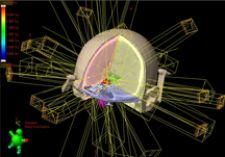
\includegraphics[width=\linewidth]{figures/boo-eclipse.jpg}
		\end{column}
		\-
		\begin{column}{0.5\textwidth}
			\centering
			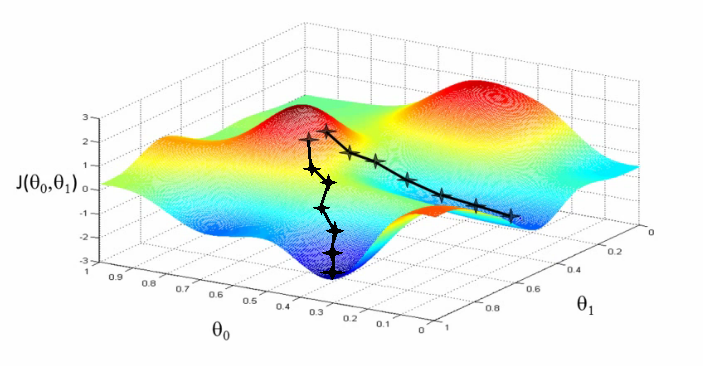
\includegraphics[width=\linewidth, height=.8\linewidth]{../Proposal/figures/nonconvex.png}
			\\
			\tiny Reprinted from David Shepard's AAPM Slides
		\end{column} 
	\end{columns} 
	%
	\begin{itemize}
		\item \small Beamlets from photons; optimal beam angles; FMO process $\rhd$ intensity modulation  
	\end{itemize}
\end{frame}

\begin{frame}
\frametitle{Existing Approaches}
\begin{itemize}
		\small
		\item Stochastic optimization approaches (SA, GA): ~\cite{ Bortfeld1993, Sodertrom1993,Pugachev2000,Pugachev02,Aleman08, Bertsimas2013}
		%
		\vspace{0.1in}
		%
		\item Gradient search:~\cite{Stein97, Craft2007, Bertsimas2013}
		%
		\vspace{0.1in}
		%
		\item Feature-based machine learning:~\cite{lu2006learning, li2010feasible}
		%
		\vspace{0.1in}
		%
		\item Mixed-integer LP, branch and cut, beam angle elimination algorithms: ~\cite{wang2003optimization, dsouza, lim2007optimization,Jia2011}
\end{itemize}
\end{frame}

\subsection{Proposal Two-Player}
\begin{frame}
\frametitle{An ADP + Monte-Carlo Evaluation Proposal}
\begin{itemize}
	\item \textbf{Context}: For $180$ discretized angles in a $5$ beam plan, there are $188,956,800,000$ possible search directions
	%
	\vspace{0.1in}
	%
	\item \textbf{Proposal}
	
	\begin{itemize}
		\item Monte-Carlo game planning strategy
		%
		\vspace{0.1in}
		%
		\item Deep neural network policy: map patients geometry to beam angles
		%
		\vspace{0.1in}
		%
		\item Refine accuracy of beams selection policy with fictitious self-play~[\cite{Heinrich}] 
	\end{itemize}
\end{itemize}
\end{frame}

\begin{frame}
\frametitle{State Representation: Network Input Plane}
\includegraphics[width=.85\columnwidth]{../../../BOO/figures/new_architecture.png}
\footnotetext{\tiny Net policy: produces a subjective probability distribution about a rational decision-making agent's preference for a \textit{lottery} (or \textit{value}) in an uncertain environment. 
	%It characterizes a  policy's belief about all relevant unknown factors at the current time step $k$ given a decision $u_k$. 
With new information, decision-maker's subjective probability distribution gets revised. Repeatedly sampling from this probability distribution enables the transition between episode contexts, \ie $\state_k \rightarrow \state_{k+1}$.}
\end{frame}

\frame{
	\frametitle{Two-Player Framework}
	\begin{itemize}
		\item Players base their decisions on a random event's outcome 			
		%
		\vspace{0.1in}
		%
			\item Guided by  a nonstationary Markovian policy set $\Pi^{p_i} =  \{\Pi^{p_1},  \Pi^{p_2}\}$ such that
			%
			\begin{itemize}
			%
			\item $\policy^{p_1} \in \{\pi^{p_1}_0, \pi^{p_1}_1, \ldots, \pi^{p_1}_{T}\} \subseteq \Pi^{p_1}$
			%
			\vspace{0.1in}
			%
			\item $\policy^{p_2} \in \{ \pi^{p_2}_0, \pi^{p_2}_1, \ldots , \pi^{p_2}_{T}\} \subseteq \Pi^{p_2}$
		\end{itemize}
	%
	\vspace{0.1in}
	%
	\item  \textbf{Stochastic action selection strategy} $\policy(\action|\state) :=\{\policy^{p_1}, \policy^{p_2}\}$ contain control sequences $\{\action^{p_1}_t\}_{0 \le t \le T}$ and $\{\action^{p_2}_t\}_{0 \le t \le T}$
	\end{itemize}
}

\begin{frame}
\frametitle{Cost-to-go}
%
\begin{itemize}
	\item Optimal \textbf{cost-to-go} value function for state %$\state$ in stage $t$, with horizon length $T$ 
	%
	\begin{align}
	V_t^*(\state) & = \inf_{\pi^{p_1} \in \Pi^{p_1}} \sup_{\pi^{p_2} \in \Pi^{p_2}} \bb{E}\left[\sum_{t=i}^{T-1} V_t(\state_0, f(\state_t, \pi^{p_1}, \pi^{p_2})) \right], \nonumber \\
	&	\qquad  \state \in \textbf{X}; \, V_T^*(\state) = 0, \, \, \forall \, \state \in \textbf{X}\nonumber
	\end{align}
	%
	\item Each player % bases its decision on a random event's outcome 
	generates a \textbf{mixed strategy} determined by \textbf{averaging the outcome} of individual plays
	%
	\item  Find optimal saddle point control pair $\{\action^{p^*_1}_t, \action^{p^*_2}_t\}$ % can be recursively obtained by %optimizing a state-action value cost, $\cost_t(\netstate, \action)$ 
	%
%	\begin{align}
%	V_t^*(\state_t, \policy^{p_1}_t, \policy^{p_2}_t) &= \min_{\policy^{p_1} \in \Pi^{p_1}} \max_{\policy^{p_2} \in \Pi^{p_2}} V^\star_t(\state_t, \policy^{p_1}, \policy^{p_2})   \\
%	%
%	\, & \quad \forall \, \state_t \in \mc{S}, \policy^{p_1} \in \Pi^{p_1}, \policy^{p_2} \in \Pi^{p_2}.
%	\end{align}
such that
\[
V^\star_{p_1} \le V_t^\star \le V^\star_{p_2} \quad \forall \,  \{\pi^{p_1}_t, \pi^{p_2}_t\}_{0 \le t\le T}.
\]
%where $V^\star_{p_i}$ are the respective optimal values for each player. 
\end{itemize}
\end{frame}

\subsection{Search}
\begin{frame}
\frametitle{Game Tree Simulation}
\begin{itemize}
	\item Network roll-out policy guides a tree's game, $\Gamma$, toward a \textit{best-first} set of  beam angle candidates
	%
	\vspace{0.1in}
	%
	\item Essentially, a sampling-based lookout algorithm 
	%
	\vspace{0.1in}
	%
	\begin{itemize}
		\item Focus on state space regions with least FMO score for beam angle combinations
		%
		\vspace{0.1in}
		%
		\item Lookout simulation steps: \textbf{Selection}; \textbf{Expansion};  \textbf{Simulation}; \textbf{Back-up}
		%
		\vspace{0.1in}
		%
		\item A `best move' for current beam block  selected, after each  iteration
	\end{itemize}  
\footnotetext{\tiny \textit{Selection}: from root node,  recursively apply child selection policy to navigate tree branches  until an expandable node is encountered. \textit{Expansion}:  iteratively add one or more children to the current node, based on the available move probabilities.
}
\end{itemize}
\end{frame}

\subsection{Fluence Map Optimization}
\begin{frame}
\frametitle{Fluence Map Optimization (FMO)}
\begin{itemize}
	\item Suppose $\voxtot$ is the total discretized $VOI$'s in a target volume
	%
	\vspace{0.1in}
	%
	\item Suppose $\beamlets_1 \cup \beamlets_2 \cup \ldots \cup \beamlets_n \subseteq \beamlets$ represents the partition subset of a  beam $\beamlets$
	%
	\vspace{0.1in}
	%
	\item Suppose further that $\dij(\beamangle_k)$ is the matrix that describes each dose influence, $d_i$.
	%
	\vspace{0.1in}
	%
%	\item  $\dij(\beamangle_k)$ delivered to a discretized voxel, $i$, in a volume of interest, $VOI_h \, (h = 1, \ldots, \voxtot)$, from a beam angle, $\beamangle_k$, $k \in \{1, \ldots, n\}$
%	%
%	\vspace{0.1in}
	%
	\item $\dij(\beamangle_k)$ is computed for each dose to voxel $i$ occupying a bixel, $j$, incident from a beam angle, $\beamangle_k$ at every $360^\circ/\varphi^\circ$. NB: $j \in \beamangle_k$
\end{itemize}
\end{frame}
%
\begin{frame}
\frametitle{The FMO Problem}
\begin{itemize}
\item Pre-calculated dose term:  $\Amat\primal = \{\sum_s\frac{w_s}{v_s} \dij^s \primal_s  \, | \, \dij^s \in \bb{R}^{n \times l}, n \gg l \}$%, which is a combination of the dose components that belong to OARs and those that belong to PTVs. 
%
\vspace{0.1in}
%
\item Find decision variable $\textbf{x}_j$ that maximizes dose to tumor, and  minimizes dose to critical structures and body tissues for all $k \in \{1, \ldots, n\}$
%
\vspace{0.1in}
%
\small \begin{align}
\small 
\min \frac{1}{v_s}\sum_{s \in \text{OARs}}  &\|(b_s - \underline{w}_s \dij^s \primal_s)_+ \|_2^2 + \frac{1}{v_s}\sum_{s \in \text{PTVs}}  \|(\bar{w}_s \dij^s \primal_s - b_s)_+\|_2^2 \nonumber \\
&\quad  \text{ subject to }  \textbf{x} \ge 0. \nonumber
\end{align}
%
\item Restated as
\[
\min \frac{1}{2}\|A \textbf{x} - \textbf{b}\|_2^2  \quad \text{ subject to }  x \ge 0.
\]
\end{itemize}
\end{frame}
%
\begin{frame}
\frametitle{FMO Lagrangian}
\begin{itemize}
\item  Lagrangian:
%
\[
L(\primal, \bm{\lambda}) = \frac{1}{2}\|A \textbf{x} - \textbf{b}\|_2^2 - \bm{\lambda}^T \primal.
\]
%\item Since we are solving a large scale problem, we use the ADMM algorithm
%
\item Introduce the auxiliary variable $\textbf{z}$, we have 
\begin{align}
\min_{\primal} \frac{1}{2}\|\Amat \primal - \textbf{b}\|_2^2,
\,\,\, \text{ subject to }  \admmvar = \primal, \,\, \admmvar \ge 0, \nonumber
\end{align}
\end{itemize}
\end{frame}


\begin{frame}
\frametitle{FMO Primal and Dual Updated}
\begin{itemize}
\item Solving the $\primal$ and $\admmvar$ sub-problems, we have
%
\tcb{
\begin{align}
\primal^{k+1} &= \left(\Amat^T\Amat + \rho \bm{I}\right)^{-1}\left(\Amat^T\bm{b}+ \rho \admmvar^k - \bm{\lambda}^k\right)  \nonumber \\
%\label{eq:admm_xupdate}
%
\admmvar^{k+1} &= S_{\bm{\lambda}/\rho}\left(\primal^{k+1} + \bm{\lambda}^k \right)%,
\nonumber
\end{align}
}{$\primal,\admmvar$-updates}
%
%
where $S_{\bm{\lambda}/\rho}(\tau) = (\primal - \bm{\lambda}/\rho)_+ - (-\tau - \bm{\lambda}/\rho)_+$, and %$\bm{\lambda}$ is updated as
%
\[
\bm{\lambda}^{k+1} = \bm{\lambda}^k - \gamma (\admmvar^{k+1} - \primal^{k+1}),
\]
with $\gamma$ as the step length controlling parameter.
\end{itemize}
\end{frame}

\subsection{Results}
\newcommand{\putdose}[2]{\includegraphics[width=#2\columnwidth, height=.45\columnwidth]{../../../BOO/figures/dvh_dose/#1}}
\newcommand{\dosewidth}{.5}

\newcommand{\putdvh}[2]{\includegraphics[width=#2\columnwidth, height=.42\columnwidth]{../../../BOO/figures/dvh_dose/#1}}
\newcommand{\dvhwidth}{.5}

\begin{frame}
\frametitle{Results: Dose Wash Plot}
\begin{table}[tb!]
	\centering
	\begin{tabular}{c@{}c@{}}
		%
		\putdose{case_007/dose.png}{\dosewidth} & \putdose{case_022/dose.png}{\dosewidth}
		%
	\end{tabular}
	\label{tbl:dose}
	%
\end{table}
\end{frame}


\begin{frame}
\frametitle{Results: Dose Wash}
\begin{table}[tb!]
\centering
\begin{tabular}{c@{}c@{}}
	%
	\putdose{case_075/dose.png}{\dosewidth} & \putdose{case_077/dose.png}{\dosewidth} 
	%
\end{tabular}
\label{tbl:dose_test}
%
\end{table}
\end{frame}

%\begin{frame}
%\frametitle{Results: Clinically Optimized DVH Curve}
%\begin{columns}[c]
%	\begin{column}{.5\textwidth}
%		\includegraphics[width=\linewidth]{../../../BOO/figures/clinic_plan.png}
%	\end{column}
%	\begin{column}{.5\textwidth}
%		\includegraphics[width=\linewidth]{../../../BOO/figures/dvh_dose/case_007/dvh.png}
%	\end{column}
%\end{columns}
%\end{frame}
%
%\begin{frame}
%\frametitle{Results: Deep BOO Optimized DVH Curve}
%\begin{columns}[c]
%	\begin{column}{.5\textwidth}
%		\includegraphics[width=\linewidth]{../../../BOO/figures/dvh_dose/case_022/dvh.png}
%	\end{column}
%\begin{column}{.5\textwidth}
%\includegraphics[width=\linewidth]{../../../BOO/figures/dvh_dose/case_075/dvh.png}
%\end{column}
%\end{columns}
%\end{frame}

\begin{frame}
\frametitle{Previously Proposed Future Work (Last Fall)}
\begin{itemize}
	\item Supervised Pretraining
	%
	\vspace{0.1in}
	%
	\begin{itemize}
		\item For example, PlanIQ or Column generation to eliminate plan quality gap and save training process time
		%	
		\vspace{0.1in}
		%
		\item Kalman filtering of predictions from neural network policy to obtain stable probabilities
	\end{itemize}
	%
	\item Robust policy improvement of pre-training angle predictions 
	%	
	\vspace{0.1in}
	%
	\begin{itemize}
		\item \eg Monte-Carlo Tree Search or Graph Convolutional Networks and guided tree search~[\cite{graphConvTreeSearch}].
	\end{itemize}
\end{itemize}
\end{frame}

\begin{frame}
\frametitle{Supervised Pre-Training of Deep BOO Policy}
\centering This page is left blank intentionally.
\end{frame}

%\section{BOO II}

\begin{frame}
	\frametitle{Generative MDP Prior}
	\begin{itemize}
		\item Generative model to find near-optimal beams in large state-space MDP: ~\cite{Azar19MICCAI, AzarPMB19}
		%
%		\vspace{0.1in}
%		%
%		\item Given dose data, structure weights and currently chosen beams, a column-generation (CG) scheme maps from patients' anatomy to beam angles.
%		%
%		\vspace{0.1in}
%		%
%		\item \cite{Azar19ICCR}: A greedy beams-selection prior iteratively predicts beamlets given a current state 
%		%
%		\vspace{0.1in}
		%
	\end{itemize}
	\frametitle{Generative MDP Prior/State Representation}
\centering
\framebox{{
		\includegraphics[width=.85\columnwidth, height=0.4\columnwidth]{../../../BOO/figures/state.png}
}}
\end{frame}

%\begin{frame}
%	\frametitle{State Representation}
%		\centering
%		\framebox{{
%			\includegraphics[width=.85\columnwidth, height=0.4\columnwidth]{../../../BOO/figures/state.png}
%	}}
%\end{frame}

\begin{frame}
\frametitle{Generative MDP Prior}
\begin{itemize}
	\item For a subset  $\blim$ of discretized beams set, $B$, find  optimal beams set $\blim^\star$ via greedy linear programming strategy
	%
	\vspace{0.1in}
	%
	\item \textbf{How?}
	%
	\begin{itemize}
		\item Iteratively add beams to $\blim$ until $|\blim|$, reaches a threshold, $\bar{B}_{\text{lim}}$
		%
		\vspace{0.1in}
		%
		\item Or when the master problem's optimality condition is met
	\end{itemize}
	%
	\vspace{0.1in}
	%
	\item Add beams only if it reduces the current objective function's value from a previous iteration
	%
%	\vspace{0.1in}
%	%
%	\item Details in ~\cite{AzarPMB19}
\end{itemize}
\end{frame}

\begin{frame}
	\frametitle{Column Generation Procedure}
	\begin{itemize}
		\item A deep policy (\textit{base policy}) parameterizes the column generation functional mapping 
		%
		\vspace{0.1in}
		%
		\item Beam orientation input is a zero-initialized vector whose particular indices are complemented over the course of backpropagation
		%
		\vspace{0.1in}
		%		
		\item Base policy minimizes MSE between CG prediction, $\state_{k+1}^{cg}$, and KKT targets $\state_{k+1}^{kkt}$
		%
		\vspace{0.1in}
		%		
		\item Policy outputs a probability distribution which informs the beam index to which a new beamlet $\state_{k+1}$ is inserted at next iteration
	\end{itemize}
\end{frame}

%\begin{frame}
%	\frametitle{Sparse Lookahead Search}
%	\begin{itemize}
%		\item Denote base policy as $\{\mu_0, \ldots, \mu_{N-1}\}$ , over an horizon $N$
%		%
%		\vspace{0.1in}
%		%		
%		\item Simulated beam plans are a consequence of
%		%
%		\begin{align}
%		\state_{i+1} = f_i(\state_i, \mu_i(\state_i), w_i), \quad i =k+1, \ldots, N-1
%		\label{eq:state_eq}
%		\end{align}
%		%
%		where $\{\mu_{k+1}, \ldots, \mu_{N-1}\}$ represents the tail part of the base policy 
%		%
%		\vspace{0.1in}
%		%		
%		\item First generated state form 
%		\begin{align}
%		\state_{k+1} = f_k(\state_k, u_k, w_k)
%		\label{eq:trajectory}
%		\end{align}
%		%
%		with independent random samples $\{w_k, \ldots, w_{N-1}\}$. %~\cite{Bertsekas17DynProI}.
%	\end{itemize}
%\end{frame}

\begin{frame}
	\frametitle{Policy Recovery}
	\begin{itemize}
		\item Search task is to recover a policy $p(u_k | \state_k; \mu)$ or $\policy_\mu(\action_k|\state_k)$
		%
		\vspace{0.1in}
		%		
%		\item Simulate \textit{cost-to-go} approximation for the unknown transition probabilities and system equations~\eqref{eq:state_eq} using in part  Monte-Carlo simulations
%		%
%		\vspace{0.1in}
		%		
		\item Simulate state-action \textit{cost-to-go} approximation of running beam trajectories by drawing samples from
		%
		\begin{align}
		Q_k(\state_k, u_k) = \mathbb{E}\left[g_k(\state_k, u_k, w_k) + J_{k+1}(\state_k+1)\right]
		\label{eq:q_est}
		\end{align}
		%		
		\item Average $Q_k(\state_k, u_k)$ costs of each control $u_k \in U_k(\state_k)$ to obtain an estimate $\bar{Q}_k(\state_k, u_k)$
		%
		\vspace{0.1in}
		%
		\item Find approximate rollout control $\bar{\mu}_k(\state_k)$ from the minimization 
		\begin{align}
		\bar{\mu}_k(\state_k) = \arg \min_{u_k \in U_k(\state_k)} \bar{Q}_k(\state_k, u_k).
		\end{align}
		
	\end{itemize}
	\footnotetext{\tiny Policy distributed over controls, $u_k$,  conditioned on the states, $\state_k$, and parameterized by a rollout (tree) policy, $\mu$. $J_{k+1}(\state_k+1)$ denotes the cost of  running the base policy starting from $\state_{k+1}$, and $g_k(\state_k, u_k, w_k)$ is the cost of running the current tree policy. }
\end{frame}

\begin{frame}
	\frametitle{Monte-Carlo Tree Search Stages}
	\begin{itemize}
%		\item Repeat $t \rightsquigarrow \infty$
%		\begin{itemize}
%			\item Select $\rhd$ Expand $\rhd$ Simulate $\rhd$ Backup
%		\end{itemize}
		\item Simulate single agent games from $\state_0$ up to a fixed depth with child selection policy 
		%
%		\vspace{0.1in}
%		%
%		\item Find allocation rule for determining the state transitions 
		%
		\vspace{0.1in}
		%
		\item As search progresses towards convergence given simulation length, bound worst possible bias by a quantity that converges to zero
		%
		\vspace{0.1in}
		%
		\item Rewrite \eqref{eq:q_est} as
		\begin{align}
		\bar{\mu}_k^\star(\state_k) = \bar{\mu}_k(\state_k)n \pm \mu_j \sum_{j=1}^{K}\bb{E}[T_j(n)]
		\label{eq:regret}
		\end{align}
		%
		\item UCT single player: %following ~\cite{SPMCTS}'s recommendation
		\begin{align}
		\bar{Q}(\state_k, \action_k) = {Q}_j(\state_k, \action_k) + c_p \cdot \pi(\state_k) \sqrt{\dfrac{ln \, N_p}{1+N_c}} + \kappa% \sqrt{\dfrac{\sum x^2 - N_p {\bar{\mu}_k}^2+\kappa}{N_c}}
		%\bar{\mu}_k^\star(\state_k) = \bar{\mu}_k + c_p \sqrt{\dfrac{ln \, N_p}{N_c}} + \sqrt{\dfrac{\sum x^2 - N_p {\bar{\mu}_k}^2+\kappa}{N_c}}
		\label{eq:spmcts}
		\end{align}
	\end{itemize}
	\footnotetext{\tiny Child selection policy drawn from $\{\mu_0, \ldots, \mu_{N-1}\}$.}
\end{frame}

\newcommand{\putdosejbme}[2]{\includegraphics[width=.45\columnwidth,height=.35\columnwidth]{../../../BOO/figures_mcts/#1}}
\newcommand{\dosejbmewidth}{.45}
\begin{frame}
	\frametitle{Results: Dose distribution on select prostate cases}
	\centering
	%
	\begin{tabular}{c@{}c@{}}
		\putdosejbme{Case008/dose.png}{\dosejbmewidth} &
		\putdosejbme{Case023/dose.png}{\dosejbmewidth} 
	\end{tabular}
	%
	\begin{tabular}{c@{}c@{}}
		\putdosejbme{Case035/dose.png}{\dosejbmewidth} & 
		\putdosejbme{Case040/dose.png}{\dosejbmewidth}
	\end{tabular}
\end{frame}

\newcommand{\putdvhii}[2]{\includegraphics[width=\linewidth, height=.7\columnwidth]{../../../BOO/figures_mcts/#1}}
\begin{frame}
\frametitle{DVH curves comparison}
	\centering
	%
	\begin{columns}[c]
		\begin{column}{.5\textwidth}
			\putdvhii{Case008/dvh_7.png}{\dosewidth} 
		\end{column}
		%
		\begin{column}{.5\textwidth}
			\putdvhii{Case023/dvh_8.png}{\dosewidth} 
		\end{column}
	\end{columns}
\end{frame}

\begin{frame}
\frametitle{DVH curves comparison}
\centering
\begin{columns}[c]
	\begin{column}{.5\textwidth}
		\putdvhii{Case030/dvh_2.png}{\dosewidth} 
	\end{column}
	%
	\begin{column}{.5\textwidth}
		\putdvhii{Case035/dvh_5.png}{\dosewidth} 
	\end{column}
\end{columns}
\end{frame}

\begin{frame}
\frametitle{DVH curves comparison}
	\centering
	%
	\begin{columns}[c]
		\begin{column}{.5\textwidth}
			\putdvhii{Case040/dvh_2.png}{\dosewidth} 
		\end{column}
		%
		\begin{column}{.5\textwidth}
			\putdvhii{Case057/dvh_9.png}{\dosewidth} 
		\end{column}
	\end{columns}
\end{frame}

\begin{frame}
\frametitle{DVH curves comparison}
\centering
%
\begin{columns}[c]
	\begin{column}{.5\textwidth}
		\putdvhii{Case087/dvh_9.png}{\dosewidth}
	\end{column}
	%
	\begin{column}{.5\textwidth}
		\putdvhii{Case091/dvh_1.png}{\dosewidth} 
	\end{column}
\end{columns}
\end{frame}

\section{Future Work}

% ---- Bibliography ----
\bibliographystyle{../../Proposal/styles/bibtex/spmpsci_unsrt}
{
\tiny
\bibliography{../../../PhDThesis/chapters/biblio}
}
\end{document}
